\documentclass[12pt, a4paper]{article}

\usepackage[utf8]{inputenc}
\usepackage[T1]{fontenc}
\usepackage{lmodern}   % vector Latin Modern fonts; replaces bitmap EC fonts under T1
\usepackage[english]{babel}
\usepackage{geometry}
\usepackage{setspace}
\usepackage{booktabs}
\usepackage{array}
\usepackage{tabularx}
\usepackage{longtable}
\usepackage{amsmath}
\usepackage{amssymb}
\usepackage{hyperref}
\usepackage{graphicx}
\usepackage{float}
\usepackage{parskip}
\usepackage{titlesec}
\usepackage{tocloft}
\usepackage{fancyhdr}

\usepackage{enumitem}
\usepackage{xcolor}

\geometry{
  top=2.5cm,
  bottom=2.5cm,
  left=3cm,
  right=2.5cm
}

\hypersetup{
  colorlinks=true,
  linkcolor=black,
  citecolor=black,
  urlcolor=blue,
  hypertexnames=false
}

% Section formatting
\titleformat{\section}{\large\bfseries}{\thesection}{1em}{}
\titleformat{\subsection}{\normalsize\bfseries}{\thesubsection}{1em}{}
\titleformat{\subsubsection}{\normalsize\bfseries}{\thesubsubsection}{1em}{}
\setcounter{tocdepth}{2}

\setlength{\parindent}{0pt}
\setlength{\parskip}{6pt}
\graphicspath{{figures/}}

% Header/footer
\pagestyle{fancy}
\fancyhf{}
\fancyfoot[C]{\thepage}
\renewcommand{\headrulewidth}{0pt}

\begin{document}

% ============================================================
%  TITLE PAGE
% ============================================================
\begin{titlepage}
\newpage

{\setstretch{1.1}
\begin{center}
\textbf{National Research University Higher School of Economics}\\[12pt]
\textbf{Faculty of Computer Science}\\[2pt]
\textbf{Programme: Data Science and Business Analytics}
\end{center}
}

\vspace{5em}

\begin{center}
\textbf{BACHELOR'S THESIS}\\[6pt]
\textbf{Research Project}\\[6pt]
\textbf{Algorithms with Predictive Models for Autonomous Navigation of Mobile Robots in Dynamic Environments}
\end{center}

\vspace{5em}

\textbf{Prepared by the student of Year 4, Faculty of Computer Science,}\\
\textbf{Belikov Daniil Maksimovich}

\vspace{2em}

\textbf{Thesis Supervisor:}\\
\textbf{PhD in Computer Science, Dergachev Stepan Alekseevich,}\\
\textbf{Basic Department of the Federal Research Center ``Informatics and Control''}

\vspace{\fill}

\begin{center}
\textbf{Moscow, 2026}
\end{center}
\end{titlepage}

% ============================================================
%  TABLE OF CONTENTS
% ============================================================
\tableofcontents
\newpage

% ============================================================
%  GLOSSARY / NOTATION
% ============================================================
\section*{Key Definitions, Notation, and Abbreviations}
\addcontentsline{toc}{section}{Key Definitions, Notation, and Abbreviations}

\textbf{Abbreviations.}

\begin{tabular}{ll}
ADE & Average Displacement Error \\
CNN & Convolutional Neural Network \\
CV & Constant Velocity (model) \\
CVAE & Conditional Variational Autoencoder \\
FDE & Final Displacement Error \\
GAN & Generative Adversarial Network \\
GRU & Gated Recurrent Unit \\
HD map & High-Definition map \\
MLP & Multi-Layer Perceptron \\
MPC & Model Predictive Control \\
MPPI & Model Predictive Path Integral (control) \\
Nav2 & ROS\,2 Navigation Stack \\
ROS\,2 & Robot Operating System, version 2 \\
SARL & Socially Attentive Reinforcement Learning \\
VAE & Variational Autoencoder \\
\end{tabular}

\textbf{Key notation.}

\begin{tabular}{ll}
$\mathbf{x}_t,\mathbf{u}_t$ & Robot state and control input at time $t$ \\
$\mathbf{U}_k$ & Planned control sequence at planning tick $k$ \\
$H$ & MPPI/prediction horizon (steps) \\
$L$ & Pedestrian observation length (steps) \\
$\mathbf{p}^{i}_t$ & Observed 2D position of pedestrian $i$ at time $t$ \\
$\hat{\mathbf{p}}^{i}_h$ & Predicted position of pedestrian $i$ at horizon step $h$ \\
$\mathcal{N}^{i}_k$ & Set of neighbours of pedestrian $i$ at tick $k$ \\
$\mathcal{M}$ & Local cost map / occupancy information \\
$f_\theta(\cdot)$ & Pedestrian-motion predictor with parameters $\theta$ \\
$S(\tau_k)$ & Total cost of a sampled MPPI rollout $\tau_k$ \\
$S_{\mathrm{human}}$ & Dynamic-human cost term used by the MPPI critic \\
$\rho(\cdot)$ & Repulsive penalty on robot--human distance \\
$\alpha,\beta_s$ & Residual influence coefficient; exponential-smoothing factor \\
$g$ & Turn-activated gate of the residual predictor \\
\end{tabular}

\textbf{Key terms.} \emph{Closed-loop / open-loop evaluation}: closed-loop measures the predictor's effect on a full navigation episode; open-loop measures only its displacement error on a fixed observation window. \emph{Inter-query jitter}: distance between predictions produced at two consecutive planning ticks for the same absolute future time. \emph{Robot influence force}: scalar fed to HuNavSim that controls how strongly simulated pedestrians avoid the robot.

\newpage

% ============================================================
%  ABSTRACT
% ============================================================
\section*{Abstract}
\addcontentsline{toc}{section}{Abstract}

This thesis studies local navigation of a mobile robot in dynamic pedestrian environments and asks whether a learned correction of a constant-velocity Kalman predictor can improve a Model Predictive Path Integral (MPPI) planner without breaking the temporal stability that closed-loop control requires. A simulation pipeline based on HuNavSim, Gazebo, and ROS\,2 / Nav2 is used to collect $\approx 30{,}000$ pedestrian trajectories across three geometrically distinct scenes and to evaluate four predictors: a Kalman baseline, a Social GRU, a pre-trained SocialVAE, and a proposed Kalman + residual hybrid with neighbour encoding and a CNN cost-map branch. Predictors are compared on ADE/FDE and on streaming stability metrics (inter-query jitter, prediction jerk, acceleration error), and then in paired Wilcoxon closed-loop MPPI experiments. The main finding is that the linear Kalman filter is surprisingly hard to outperform in the full navigation loop, because its smooth, bounded outputs match what MPPI needs; the stabilized residual hybrid improves offline accuracy and yields paired-test improvements in path length, minimum agent distance, and violation time in non-reactive crowds, while in robot-reactive crowds it nominally reduces collisions without degrading the other metrics. For socially aware robot navigation, prediction stability inside the control loop is at least as important as raw offline accuracy.

\newpage

% ============================================================
%  1. INTRODUCTION
% ============================================================
\section{Introduction}

\subsection{Motivation and Problem Statement}

Autonomous mobile robots are increasingly expected to operate in environments shared with humans, including corridors, warehouses, campuses, hospitals, and service spaces (Fig.~\ref{fig:intro_motivation}). In such settings, navigation cannot be reduced to static path planning.

\begin{figure}[H]
\centering
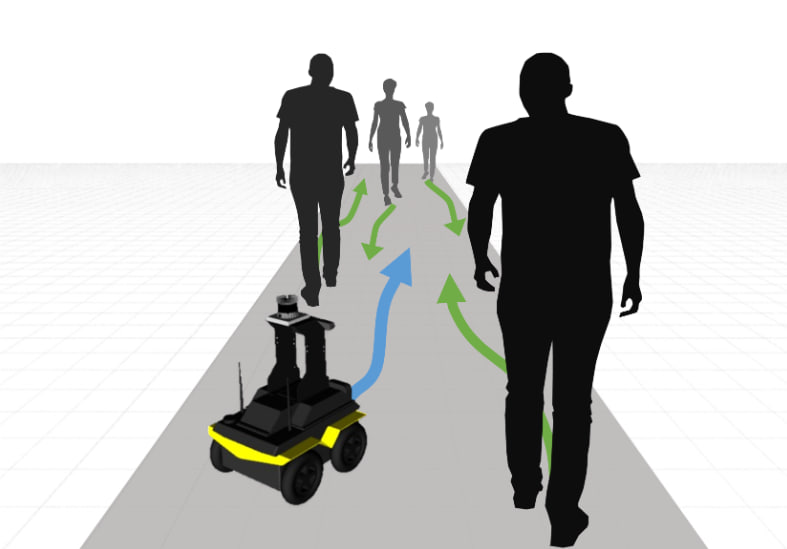
\includegraphics[width=0.7\linewidth]{intro_motivation.jpg}
\caption{An example of socially aware robot navigation: a mobile robot plans its short-term path (blue) among pedestrians whose possible future motions (green) must be anticipated rather than only reacted to. Such interactions are typical for last-mile delivery and service robots that share corridors and sidewalks with people. Image taken from~[36].}
\label{fig:intro_motivation}
\end{figure} Pedestrians are not fixed obstacles: they move with intent, interact with one another, adapt their motion to local geometry, and may also react to the robot itself. Therefore, a robot navigating among pedestrians must jointly satisfy several requirements. It must reach its goal efficiently, avoid collisions, maintain sufficient clearance from people, and avoid behavior that appears abrupt, overly aggressive, or socially inappropriate. Prior work on socially aware navigation similarly treats crowd navigation as a problem of safe and time-efficient motion among interacting agents rather than as purely geometric obstacle avoidance~[24].

The difficulty is that the robot must make decisions before the future motion of nearby pedestrians is fully observed. A planner that only reacts to current positions may choose a path that is already unsafe a few seconds later. Conversely, a planner that assumes overly conservative future motion may stop unnecessarily or produce inefficient detours. This makes human motion prediction a core component of the navigation system rather than a separate module: the predictor determines how future pedestrian positions enter the local planner's cost function, and therefore strongly affects the robot's selected control command.

This work focuses on local navigation in pedestrian-populated dynamic environments and on the design of a prediction module that is useful inside a closed-loop controller, not only on a standalone forecasting benchmark. The central hypothesis is that the usefulness of a pedestrian predictor for robot navigation is not determined only by its open-loop displacement error: a predictor that achieves lower Average Displacement Error or Final Displacement Error may still degrade navigation if it changes its predictions abruptly between consecutive planning ticks, or if it produces trajectories that are inaccurate near potential conflict zones. The specific local planner used throughout the thesis is the Model Predictive Path Integral (MPPI) controller, which is introduced together with classical alternatives in the next subsection.

\subsection{Current State of the Art}

Classical local planners for mobile robots include the Vector Field Histogram (VFH)~[33], the Dynamic Window Approach (DWA)~[34], and gradient-based Model Predictive Control (MPC) in its various forms. VFH builds a polar histogram of nearby obstacles and selects a steering direction with low occupancy; it is fast and easy to deploy but treats obstacles geometrically and does not natively reason about future motion. DWA samples feasible $(v,\omega)$ pairs inside the robot's reachable velocity window and scores them by a fixed cost; it handles dynamic feasibility well but its short look-ahead and rigid cost function make it brittle in dense pedestrian traffic. Classical gradient-based MPC formulations require differentiable, typically convex cost functions and analytical Jacobians, which makes it hard to combine many heterogeneous safety and social terms in a single optimization. The Model Predictive Path Integral (MPPI) controller~[10, 25] avoids these restrictions by sampling thousands of noisy control sequences, rolling them out through the robot dynamics, evaluating arbitrary scalar costs, and forming an importance-weighted control update. This makes MPPI especially attractive when the cost function must combine global path following, static obstacle avoidance, control smoothness, and a dynamic human-proximity term simultaneously. The Nav2 MPPI controller~[26] is a recent ROS\,2 implementation of this idea with plugin-based critics, and risk-aware variants such as U-MPPI~[12] and C2U-MPPI~[27] add explicit uncertainty propagation and chance constraints over predicted obstacle distributions. In a dynamic environment every sampled robot trajectory must be scored against \emph{predicted} pedestrian positions, so the prediction module participates in every MPPI control cycle and its temporal behaviour directly affects closed-loop control.

A natural starting point for pedestrian prediction is the constant-velocity Kalman filter~[35]. It assumes that a pedestrian approximately continues with the currently estimated velocity, with Gaussian process and observation noise. Despite this simplicity, it has two properties that are highly valuable inside a navigation loop. First, it is temporally consistent: the recursive state estimate makes consecutive predictions change smoothly. Second, it is computationally negligible and requires no training data, making it robust to scene changes and easy to deploy in real time. This baseline should not be treated as weak: prior work has shown that simple constant-velocity models can match or outperform more complex neural pedestrian prediction models under common benchmark protocols~[28]. Its limitation is also clear: the constant-velocity assumption breaks down when pedestrians turn, stop, avoid other people, or react to the robot, which are exactly the cases that matter in narrow corridors, intersections, and dense interaction zones. The main question addressed in this thesis is whether the systematic errors of the Kalman predictor can be corrected by a learned residual model without losing the temporal stability that makes it effective in closed-loop navigation.

Beyond the Kalman baseline, the machine learning community has produced a series of increasingly powerful pedestrian-trajectory prediction models: recurrent architectures with social pooling~[1, 2], conditional variational autoencoders with graph structure~[3], spatio-temporal graph convolutional networks~[4, 7], transformer-based approaches~[5, 14, 15], and stochastic timewise latent-variable models~[32]. These models achieve strong ADE and FDE scores on standard benchmarks such as ETH/UCY~[11]. However, deploying them inside a real navigation pipeline introduces a different set of challenges. Models trained on pedestrian datasets collected in specific outdoor environments may fail to generalize to new indoor geometries, densities, or walking-speed distributions. More fundamentally, even a model that is accurate on its training domain may generate temporally inconsistent predictions because it is optimized for average displacement error on fixed observation windows rather than for smooth state estimation over time. Existing work has shown that better forecasting metrics do not necessarily translate into better robot navigation performance~[9, 23], motivating the system-level evaluation adopted in this thesis. Experiments here confirm that this temporal instability is a real obstacle to deploying learned predictors inside MPPI.

\subsection{Object, Goal, Tasks, and Scientific Novelty}
\label{sec:objgoaltask}

\textbf{Object of research.} The local navigation pipeline of a mobile robot operating in dynamic pedestrian environments, with focus on the human-motion prediction module of the MPPI controller in the ROS\,2 / Nav2 stack.

\textbf{Subject of research.} The relationship between properties of a pedestrian-trajectory predictor (open-loop accuracy, temporal stability, environment awareness) and the resulting closed-loop navigation behaviour of an MPPI planner.

\textbf{Goal.} To design, implement, and empirically validate a stable hybrid prediction method that improves MPPI-based robot navigation in pedestrian environments without sacrificing the temporal consistency required for real-time control.

\textbf{Tasks.} (1) Build a reproducible simulation pipeline on HuNavSim + Gazebo + ROS\,2 / Nav2 with controllable pedestrian reactivity; (2) collect pedestrian-trajectory datasets across geometrically distinct scenes and construct an offline prediction benchmark of $\approx 30{,}000$ trajectories; (3) introduce streaming stability metrics (inter-query jitter, prediction jerk, acceleration error) suitable for evaluating predictors inside an MPPI loop; (4) develop a Kalman-residual predictor with neighbour and cost-map context, together with a stabilization pipeline (turn gate, influence coefficient, exponential smoothing, clipping); (5) carry out paired closed-loop comparisons in non-reactive and robot-reactive crowd settings; (6) analyse how robot influence changes the pedestrian-motion distribution and which predictor properties matter most under each regime.

\textbf{Methods and methodology.} Sampling-based stochastic optimal control (MPPI); recursive Bayesian filtering (constant-velocity Kalman); deep learning for pedestrian-trajectory prediction (Social GRU trained on Trajectron++ data, pre-trained and fine-tuned SocialVAE, custom Kalman-residual MLP with CNN cost-map branch); simulation-based evaluation in HuNavSim + Gazebo + ROS\,2 / Nav2; paired statistical testing with the Wilcoxon signed-rank test for closed-loop navigation metrics.

\textbf{Source data and prerequisites.} The Trajectron++~[3] preprocessed ETH/UCY dataset for the Social GRU baseline; the pre-trained SocialVAE checkpoint on the HOTEL scene of ETH/UCY~[11, 32]; pedestrian trajectory logs collected in this work from HuNavSim simulations in three custom scenes (long corridor, nonlinear corridor, labyrinth) under both non-reactive and robot-reactive interaction modes.

\textbf{Planned scientific results and novelty.} (i) Empirical demonstration that for an MPPI-based robot planner, the temporal stability of a pedestrian predictor is at least as important as its open-loop accuracy, with concrete streaming metrics that capture failure modes invisible to ADE/FDE. (ii) A lightweight Kalman-residual predictor that is $\approx 16$ times smaller than a comparable SocialVAE while reaching comparable or better closed-loop behaviour. (iii) A paired closed-loop benchmarking protocol in HuNavSim + Nav2 MPPI under controlled robot-reactivity, jointly evaluating offline prediction quality, prediction stability, distribution shift, and navigation outcomes.

\subsection{Research Objectives and Contributions}

The thesis makes three main contributions.

\textbf{1. A stability-aware evaluation of prediction for MPPI navigation.} ADE and FDE alone do not reliably predict closed-loop navigation quality. A spatially accurate predictor can still destabilize the MPPI cost field through high inter-query jitter, large prediction jerk, or overconfident near-robot forecasts. This work introduces and uses streaming stability metrics alongside standard ADE/FDE.

\textbf{2. A lightweight Kalman-residual predictor.} Instead of replacing the Kalman filter, a small MLP learns a gated residual correction with map and neighbor context, followed by smoothing and clipping for runtime stability. The model is approximately 16 times smaller than the fine-tuned SocialVAE baseline and fast enough to run inside the navigation loop, while reaching comparable or better closed-loop behavior in the tested settings.

\textbf{3. Closed-loop evidence through paired MPPI experiments.} The stabilized residual model achieves paired-test gains in non-reactive navigation (path length $p=0.005$, minimum distance $p=0.029$, violation time $p=0.011$), and the robot-reactive comparison reveals why that setting is harder: robot influence changes the pedestrian data distribution and reduces the margin available for improvement over Kalman.

These contributions are supported by a simulation pipeline built on HuNavSim, Gazebo, ROS2, and Nav2 MPPI; pedestrian trajectory datasets collected across three geometrically distinct environments; robot-aware logs recorded under a controlled robot social-force scale; and a custom Nav2 MPPI critic that consumes predicted pedestrian paths. The chapter outline that maps these contributions onto the structure of the document is given at the end of Section~\ref{sec:objgoaltask}.

% ============================================================
%  2. RELATED WORK
% ============================================================
\section{Related Work}
\label{sec:related}

\subsection{Local Planners for Pedestrian Environments}

Several distinct families of local planners have been used for robot navigation in pedestrian-populated environments, and MPPI is only one of them. Classical reactive methods such as the Vector Field Histogram (VFH)~[33] and the Dynamic Window Approach (DWA)~[34] choose a control by scoring a small set of feasible velocities or steering directions against a fixed cost; they are computationally cheap and widely deployed, but their short look-ahead makes them brittle in dense pedestrian traffic, and they treat people as instantaneous obstacles rather than as agents with future motion. The Timed Elastic Band (TEB) family of methods refines a continuous trajectory under explicit kinodynamic constraints, but classical gradient-based Model Predictive Control variants on which it relies typically require differentiable, often convex, cost functions and analytical Jacobians, which makes it hard to combine many heterogeneous safety and social terms in a single optimization. End-to-end learned navigation policies based on deep reinforcement learning, such as SARL~[17] and CrowdNav~[18], bypass the explicit prediction problem and learn a control policy directly from interaction; they can produce socially natural behaviour but sacrifice interpretability and the ability for an operator to directly control risk tolerance. Recent learning-based MPC formulations~[22, 23] couple Social-LSTM-style prediction with model predictive control and have shown that the predictor-planner combination can be beneficial when the predictor is used in a way that matches the control objective.

MPPI~[10, 25, 26] sits between these families: it preserves the optimization structure of classical MPC but, by sampling rollouts and weighting them by arbitrary scalar costs, avoids the differentiability and convexity restrictions that limit gradient-based MPC. This is what makes it possible to combine global path following, static obstacle avoidance, control smoothness, and a dynamic human-proximity term inside one optimization. The remainder of this subsection focuses on what is specific to the Related Work view of MPPI: how recent extensions handle uncertainty in the forward model, and why pedestrian prediction remains a bottleneck even after these extensions.

Two risk-aware extensions are directly relevant to this work. U-MPPI~[12] incorporates the Unscented Transform to propagate uncertainty through the cost evaluation, enabling the planner to account for prediction uncertainty in a principled way. C2U-MPPI~[27] builds on U-MPPI by adding chance constraints that bound the probability of constraint violations under the predicted distribution of obstacle positions. These extensions demonstrate that even when the control side is made more sophisticated, the quality of the human motion predictor remains a fundamental bottleneck: a planner that propagates uncertainty correctly is only as accurate as the predictive distribution it is given. Improving prediction is therefore complementary to, rather than redundant with, improving the planner.

The authors of~[13] survey sampling-based MPC methods for autonomous systems and highlight the dependence of all such methods on the accuracy and consistency of the forward model used to evaluate candidate trajectories. This dependence is particularly acute when the forward model includes predictions of other agents' motions, because errors in those predictions directly corrupt the cost landscape on which the optimizer operates. The social-navigation setting adds a second difficulty that does not appear in static navigation: in a crowd, every candidate rollout is evaluated against a moving cost field induced by pedestrian forecasts rather than a fixed cost map. This makes MPPI sensitive to the temporal consistency of the predictor --- if the same pedestrian's future position changes sharply between adjacent control cycles, the optimizer may switch between different local minima even when the observed human motion itself is smooth. This observation is the main reason why this thesis treats stability as a property of the prediction module rather than as a post-processing detail, and it directly motivates the streaming-stability metrics introduced in Section~\ref{sec:stabilization}.

\subsection{Pedestrian Trajectory Prediction}

The problem of predicting pedestrian trajectories has been studied extensively. Before the deep-learning era, recursive Bayesian filters were the dominant approach. The constant-velocity Kalman filter~[35] in particular remains the standard low-complexity tracker for pedestrian-like targets and is still used as the baseline predictor in many multi-object tracking and crowd-navigation pipelines. Recent work has even shown that, when carefully tuned, a constant-velocity model can match or outperform much more complex neural pedestrian predictors under common benchmark protocols~[28]. This makes it an essential reference point rather than a weak straw man.

The foundational Social LSTM paper~[1] showed that recurrent neural networks with a social pooling mechanism, which aggregates hidden states among nearby pedestrians, can capture interaction-dependent motion patterns and significantly outperform constant-velocity baselines on the ETH/UCY benchmark. Social LSTM introduced the idea that trajectory prediction should be a joint problem over all visible agents rather than a collection of independent single-agent forecasts.

Social GAN~[2] extended the social pooling idea by replacing the LSTM decoder with a generative adversarial network, enabling the model to produce a diverse set of socially acceptable future trajectories rather than a single deterministic prediction. The use of a discriminator trained to distinguish real trajectories from generated ones encourages physically plausible and socially consistent predictions, and the paper also proposed the FDE metric as a way to evaluate whether at least one of the model's samples is close to the ground truth.

Trajectron++~[3] provides a graph-structured recurrent model that explicitly conditions the prediction on the dynamics and types of all surrounding agents as well as on a semantic map of the environment. It uses a Conditional Variational Autoencoder to generate a distribution over future trajectories, which is important for safety-critical applications where worst-case outcomes matter alongside average ones. The semantic map conditioning is directly related to the motivation for including a cost map branch in the residual model proposed in this work.

Transformer-based architectures have more recently achieved state-of-the-art results on trajectory prediction benchmarks. AgentFormer~[14] uses a time-space transformer that models temporal and social correlations jointly, enabling the model to attend to relevant agents at the relevant timesteps simultaneously. STGAT~[15] combines graph attention networks with LSTMs to model spatial interaction graphs and has shown strong performance on crowded pedestrian datasets. These architectures motivate the choice of neighbor-aware input representations in the residual model used here. ForceFormer~[5] combines transformer-based encoding with the physics-inspired social force model, arguing that explicitly representing repulsive and attractive forces between agents provides a useful inductive bias. A related line of work by Mohamed et al.~[7] proposes a spatiotemporal graph convolutional network (STGCN) that models spatial relationships through graph convolutions and temporal dynamics through standard convolutions, showing improvements in computation time and scalability over recurrent architectures.

A recurring theme is the difficulty of generalizing learned models to new settings. Yao et al.~[8] address this with a self-supervised continual learning approach that adapts the predictor to unseen pedestrian dynamics without requiring new labeled data and without catastrophically forgetting previously learned behavior. This work is particularly relevant because domain shift, the mismatch between the distribution seen during training and that encountered during deployment, is precisely the problem observed when deploying pre-trained models inside the simulation environment used here.

A parallel line of work goes beyond social interaction and adds static environment context to the predictor. Casas et al.~[16] show that incorporating high-definition maps into the predictor substantially reduces errors in scenarios where the road geometry constrains the set of plausible future trajectories. While their work targets autonomous driving rather than pedestrian navigation, the principle directly motivates the CNN-based cost map encoding used in the residual model proposed here, which allows the predictor to reason about which predicted trajectories are physically possible given the static environment. Sadeghian et al.~[20] propose SoPhie, which uses a GAN-based generator conditioned on both social interaction features and scene-level features extracted from a top-down image of the environment via a convolutional encoder; the scene encoder allows the model to avoid predicting trajectories that pass through walls or other static obstacles, which is especially important in indoor environments with complex layouts. The CNN cost-map branch in the residual model used in this work is motivated by the same principle, applied to the local occupancy representation available from the robot's navigation stack rather than to a global semantic image.

\subsection{The Prediction--Navigation Gap}

A critical but underappreciated question is whether improvements in offline trajectory prediction metrics actually translate into improvements in robot navigation performance. Poddar et al.~[9] study this question directly and show that the relationship is not straightforward: a model with better ADE may produce worse navigation outcomes if its predictions are less consistent over time or if their distribution is poorly calibrated relative to the planner's cost function. This work strongly motivates the focus on temporal stability as a first-class evaluation criterion throughout this thesis.

More recent work makes this problem even clearer. Poddar et al.~[9] show that transferring a learned crowd motion predictor into robot navigation is non-trivial: a Social-GAN-style predictor can improve open-loop forecasting quality without producing a clear navigation advantage over a constant-velocity baseline. Conversely, work that tightly couples Social-LSTM-style prediction with MPC demonstrates that prediction and planning can be beneficial when the predictor is used in a way that matches the control objective~[22]. Trajectron++ also emphasizes that forecasting models can be conditioned on ego-agent motion plans, which is directly relevant when pedestrians react to the robot's own motion~[3]. Recent learning-based MPC studies similarly report a discrepancy between open-loop prediction improvement and closed-loop navigation performance, motivating system-level evaluation rather than relying on ADE/FDE alone~[23].

The present work follows this line but narrows the question to an MPPI/Nav2-style pipeline. The goal is not simply to repeat the observation that open-loop prediction quality is not identical to navigation quality. Instead, the experiments analyze concrete properties that make a predictor controller-compatible or controller-incompatible: inter-query jitter, prediction jerk, acceleration error, residual magnitude, and risk-aware errors near the robot. These properties determine how the predicted trajectories are converted into the dynamic cost field seen by MPPI.

SARL~[17] demonstrates that attention-based deep reinforcement learning can produce socially aware navigation policies that avoid crowds more naturally than purely geometric planners. By learning a policy end-to-end, SARL bypasses the explicit prediction problem but sacrifices interpretability and the ability for the operator to directly control risk tolerance. Subsequent work in the crowd-aware navigation literature, including CrowdNav~[18] and its extensions, has largely followed this end-to-end paradigm. The work of Rudenko et al.~[19] provides a comprehensive survey and analysis of pedestrian motion prediction methods evaluated specifically in the context of robot navigation; the survey identifies temporal consistency and cross-domain generalization as the two most important properties for practical deployment, a conclusion strongly confirmed by the experiments in this thesis.

\subsection{Simulation Platforms}

Experimental evaluation is a central difficulty in human-aware robot navigation. Real-world experiments with pedestrians are expensive, difficult to reproduce, and potentially unsafe when testing early-stage navigation algorithms. At the same time, purely offline trajectory prediction benchmarks are insufficient for evaluating navigation performance, because they do not include the closed-loop interaction between the robot, the planner, and surrounding humans. For this reason, simulation platforms are widely used to develop and compare navigation algorithms in dynamic human-populated environments.

Existing simulation platforms differ in their main design goals. Arena-Rosnav~[21] is an example of a general development and benchmarking platform for robot navigation in highly dynamic environments. It provides unified interfaces for adding planners, simulators, and evaluation modules, making it suitable for comparing classical, learning-based, and reinforcement-learning navigation methods under a common interface. However, such broad benchmarking frameworks are heavier than necessary when the goal is to tightly control individual pedestrian behavior and collect detailed trajectory logs for prediction experiments. SocNavBench~[29] focuses specifically on social navigation evaluation, providing photo-realistic simulation, curated episodic scenarios based on real-world pedestrian data, and a set of standardized metrics; this addresses the problem that many social navigation methods are evaluated using custom scenarios and incompatible metrics, but it is less directly suited to this thesis where the main requirement is to generate controlled robot-aware and robot-unaware pedestrian trajectories.

Crowd simulators such as MengeROS and Pedsim-style systems are also commonly used for robot navigation research~[30]. These tools are useful because standard robot simulators such as Gazebo or Stage do not by themselves provide realistic crowd behavior. MengeROS connects the Menge crowd simulator with ROS in order to evaluate robot navigation algorithms under comparable crowd conditions. This class of tools is important because it separates pedestrian behavior generation from the robot navigation stack, but additional integration work is often required when using modern ROS2/Nav2 pipelines or when detailed control over human behavior modes is needed.

HuNavSim is particularly well aligned with the goals of this thesis. It is an open-source ROS2 human navigation simulator designed for benchmarking human-aware robot navigation~[31]. It can be used together with robotics simulators such as Gazebo and provides configurable human-agent navigation behaviors in scenarios with mobile robots. This is important for the present work because the experimental design requires not only dynamic pedestrians, but also explicit control over whether pedestrians react to the robot. HuNavSim makes it possible to compare a non-reactive setting, where humans ignore the robot, with a reactive setting, where the robot contributes to the social-force dynamics of nearby pedestrians. A further advantage of the chosen setup is controllability: the experiments in this work require several controlled variations (different scene geometries, different levels of robot influence, repeated paired navigation trials, and near-robot trajectory extraction for prediction training), and HuNavSim provides these controls while remaining compatible with the ROS2/Nav2 ecosystem.

\subsection{Research Gap}

The literature reviewed above shows substantial progress in three related directions: sampling-based MPC for robot control, learned pedestrian trajectory prediction, and simulation-based evaluation of social navigation. However, these directions are still not fully connected in a way that directly solves the problem addressed in this thesis. The remaining gap is not simply the absence of a more accurate pedestrian predictor. The main gap is the lack of a prediction method that is accurate, stable, environment-aware, and demonstrably useful inside a closed-loop MPPI navigation system. Six concrete sub-gaps motivate the experimental design.

\emph{(1) Offline accuracy vs.\ downstream navigation.} Most trajectory prediction models are optimized and evaluated using ADE and FDE. These metrics measure geometric closeness to the ground-truth future trajectory, but they do not measure whether the prediction improves the decisions of a robot planner. Prior work has shown that this transfer is nontrivial: a strong learned crowd prediction model can improve motion prediction accuracy while producing little or no improvement in navigation performance compared with a simple constant-velocity baseline~[9]. This directly motivates the central evaluation principle of this thesis: prediction models intended for robot navigation must be evaluated at the system level, not only as standalone forecasting models.

\emph{(2) Temporal stability.} A local planner such as MPPI repeatedly replans at a high frequency, consuming a sequence of forecasts produced at consecutive planning ticks. Standard ADE and FDE do not penalize large changes between consecutive predictions if each individual prediction is close to the future ground truth. In a closed-loop controller, however, such inter-query instability can change the cost landscape abruptly and lead to oscillatory or overly conservative robot behavior. This thesis treats prediction stability as a first-class requirement and uses metrics such as inter-query jitter and prediction jerk to capture failure modes that are invisible in standard benchmarks.

\emph{(3) The role of simple baselines.} Many learned pedestrian forecasting methods compare against constant-velocity or Kalman-style predictors, but these baselines are often treated as weak. This assumption is not always justified. Prior work has shown that a simple Constant Velocity Model can outperform more complex neural models in pedestrian motion prediction under common benchmark settings~[28]. In robot navigation, this baseline is even stronger because it is smooth, cheap, and robust to domain shift. The challenge is therefore not merely to outperform Kalman in ADE/FDE, but to correct its systematic nonlinear errors without sacrificing its temporal consistency.

\emph{(4) Environment awareness.} Modern trajectory prediction models increasingly incorporate scene context. SoPhie uses social and physical attention over agent trajectories and top-view scene images to generate socially and physically plausible paths~[20]. Trajectron++ incorporates heterogeneous data such as semantic maps and is explicitly designed to be integrated with robotic planning and control frameworks~[3]. However, these methods are usually evaluated on offline trajectory datasets and often assume access to global semantic maps or dataset-specific scene representations. In a mobile robot navigation stack, the available environmental representation is typically a local occupancy or cost map derived from onboard sensing.

\emph{(5) Robot-reactive pedestrians.} Many prediction benchmarks model pedestrians independently of the robot, or use recorded human trajectories in which the robot is absent. In real navigation, however, pedestrians may react to the robot, and their future motion can depend on the robot's own planned or executed motion. This creates a coupled human-robot prediction problem. A predictor trained on robot-unaware trajectories may systematically fail when deployed in a robot-reactive crowd. The need for prediction models that can be conditioned on ego-agent motion plans is recognized in works such as Trajectron++~[3], but this remains difficult to evaluate in a reproducible navigation pipeline.

\emph{(6) Integrated benchmarking.} Platforms such as Arena-Rosnav and SocNavBench provide important tools for standardized evaluation, while HuNavSim provides detailed ROS2-compatible human-agent simulation~[21, 29, 31]. However, there is still a need for experimental protocols that jointly evaluate offline prediction quality, prediction stability, distribution shift under robot influence, and closed-loop navigation performance. In particular, robot-reactive simulation can change the distribution of observed pedestrian motion near the robot, increasing the frequency of turns, stop-go behavior, dense interactions, or avoidance maneuvers. A prediction method that works under one interaction regime may not transfer to another.

This thesis addresses these six gaps by studying pedestrian prediction as an internal component of MPPI navigation rather than as an isolated forecasting task. The proposed Stable Hybrid Prediction for MPPI Navigation approach keeps the Kalman filter as a stable baseline and learns a residual correction for cases where constant-velocity prediction is systematically wrong. The method incorporates local environment information through a cost-map branch, uses neighboring agents and robot-related features when available, and is evaluated using both offline prediction metrics and closed-loop navigation metrics. The resulting experimental design is intended to answer not only whether the learned predictor is more accurate, but whether it is stable and useful for the robot planner.

% ============================================================
%  3. METHOD
% ============================================================
\section{Method}
\label{sec:method}

This section is organised so that the problem statement is independent of the chosen solution method. Section~\ref{sec:problem} first states the navigation and prediction problem in a method-agnostic form. Section~\ref{sec:mppi-cost} then describes the sampling-based controller used to solve it (MPPI, with the cost function shared with the Nav2 implementation). Section~\ref{sec:baselines} presents the baseline prediction algorithms (constant-velocity Kalman filter, Social GRU, SocialVAE), and Section~\ref{sec:proposed} presents the proposed prediction algorithm based on a Kalman residual correction, together with its training objective and its stabilization pipeline.

\subsection{Problem Formulation}
\label{sec:problem}

This subsection states the navigation and prediction problem without reference to any particular solution method. It is solved by an MPPI planner in this work (Section~\ref{sec:mppi-cost}), but the same formulation could equally well be addressed by another local planner.

\paragraph{General navigation problem.} The robot operates in a known static map populated by moving pedestrians and performs local receding-horizon control. At every planning tick $k$, the robot must choose a short sequence of future controls
\[
\mathbf{U}_{k}
=
\{\mathbf{u}_{k},\mathbf{u}_{k+1},\ldots,\mathbf{u}_{k+H-1}\},
\]
where $\mathbf{u}_{t}$ is the velocity command and $H$ is the planning horizon. The controls are evaluated through the robot dynamics $\mathbf{x}_{t+1}=f(\mathbf{x}_{t},\mathbf{u}_{t})$, which produce a candidate robot rollout $\mathbf{X}_{k+1:k+H}=\{\mathbf{x}_{k+1},\ldots,\mathbf{x}_{k+H}\}$. The planner selects controls that minimize an expected trajectory cost,
\[
\mathbf{U}^{*}_{k}
=
\arg\min_{\mathbf{U}_{k}}
J(\mathbf{U}_{k}),
\]
where the cost decomposes into one term per horizon step as
\begin{align*}
J(\mathbf{U}_{k})
=
\sum_{h=1}^{H}
\Big[
&\,c_{\mathrm{goal}}(\mathbf{x}_{k+h})
+c_{\mathrm{path}}(\mathbf{x}_{k+h})
+c_{\mathrm{map}}(\mathbf{x}_{k+h})\\
&+c_{\mathrm{ctrl}}(\mathbf{u}_{k+h-1})
+c_{\mathrm{human}}(\mathbf{x}_{k+h},\mathcal{P}_{k+h})
\Big].
\end{align*}
The first terms are standard navigation objectives: progress toward the goal, agreement with the global path, avoidance of static obstacles in the cost map, and smooth feasible control. The term that makes the problem dynamic is $c_{\mathrm{human}}$, because it depends on the future positions of pedestrians $\mathcal{P}_{k+h}$. These positions are unknown at planning time and must be predicted.

\paragraph{Prediction subproblem.} At tick $k$, the robot observes recent pedestrian trajectories
\[
\mathbf{o}^{i}_{k-L+1:k}
=
\{\mathbf{p}^{i}_{k-L+1},\ldots,\mathbf{p}^{i}_{k}\},
\qquad
\mathbf{p}^{i}_{t}\in\mathbb{R}^{2},
\]
where $i$ indexes visible pedestrians and $L$ is the observation length. A predictor produces a future trajectory for each pedestrian:
\[
\hat{\mathbf{p}}^{i}_{k+1:k+H}
=
f_{\theta}\!\left(
\mathbf{o}^{i}_{k-L+1:k},\,
\mathcal{N}^{i}_{k},\,
\mathcal{M},\,
\mathbf{x}_{k}
\right),
\]
where $\mathcal{N}^{i}_{k}$ denotes nearby pedestrians and $\mathcal{M}$ denotes local map information. In the robot-aware setting, the predictor may also receive robot-relative features, because the pedestrian future is conditioned on the robot's presence and motion. The unknown future set $\mathcal{P}_{k+h}$ in the navigation objective is therefore replaced by the predicted set
\[
\hat{\mathcal{P}}_{k+h}
=
\{\hat{\mathbf{p}}^{1}_{k+h},\ldots,\hat{\mathbf{p}}^{N}_{k+h}\}.
\]
Substituting this into the full objective and collapsing the goal, path, map, and control terms into $c_{\mathrm{static}}$ gives the concrete optimization problem studied here:
\begin{align*}
\mathbf{U}^{*}_{k}
=
\arg\min_{\mathbf{U}_{k}}
\sum_{h=1}^{H}
\bigg[
&\,c_{\mathrm{static}}(\mathbf{x}_{k+h},\mathbf{u}_{k+h-1})\\
&+
\sum_{i=1}^{N}
\rho\!\left(
\left\|
\mathbf{p}^{\mathrm{robot}}_{k+h}
-
f_{\theta}^{i}(k,h)
\right\|
\right)
\bigg],
\end{align*}
where $f_{\theta}^{i}(k,h)$ denotes the predictor's estimate of pedestrian $i$ at horizon step $h$. The static and control terms are fixed once the planner has been chosen; the only component that varies between predictors compared in this thesis is the function $f_{\theta}$ inside the human-cost term.

\paragraph{Open-loop vs closed-loop properties.} A prediction error near a potential robot--human conflict directly changes the cost assigned to candidate robot trajectories. If a pedestrian is predicted too far away, unsafe rollouts receive too little penalty. If a pedestrian is predicted too close, the robot may take unnecessary detours or slow down. If the prediction jumps between consecutive planning ticks, the optimized control can also jump, even if each individual forecast has low ADE. Therefore, the goal of this work is not only to minimize open-loop displacement error
\[
\min_{\theta}\;
\frac{1}{NH}
\sum_{i=1}^{N}\sum_{h=1}^{H}
\left\|
f_{\theta}^{i}(k,h)-\mathbf{p}^{i}_{k+h}
\right\|_2,
\]
but to find a predictor that improves the navigation objective in closed loop. In practical terms, the desired predictor must be accurate enough near conflict zones, temporally stable across planning ticks, physically plausible, and conservative around the robot. This is why the experiments evaluate ADE/FDE together with navigation metrics, collision count, violation time, prediction jerk, inter-query jitter, and residual magnitude.

\subsection{Sampling-Based Controller: MPPI}
\label{sec:mppi-cost}

This subsection describes the local planner used in this work to solve the receding-horizon problem of Section~\ref{sec:problem}, and identifies the single point at which any pedestrian predictor enters it. The chosen controller is the Model Predictive Path Integral (MPPI) algorithm; the cost function structure adopted here is the same as in the Nav2 MPPI implementation~[26] used at runtime, but the discussion below is kept in the standard MPPI notation rather than the plugin-specific ``critic'' terminology.

\paragraph{Sampling and weighting.} MPPI is a receding-horizon stochastic optimal control method. At each control cycle the planner maintains a nominal sequence of future controls, samples many noisy variations of that sequence, simulates the robot motion that would result from each variation, scores every simulated trajectory, and updates the nominal sequence toward the lower-cost samples. Only the first control of the updated sequence is executed; at the next tick, the process repeats with fresh observations.

Let $x_t$ denote the robot state and $u_t$ the control input, with discrete-time dynamics $x_{t+1}=f(x_t,u_t)$. At planning time, MPPI optimizes a finite horizon of length $T$, $U=\{u_0,\ldots,u_{T-1}\}$, that should be understood as a short plan for the next few seconds rather than a complete route to the goal. The planner samples $K$ control-noise sequences
\[
\epsilon^k_{0:T-1}
=
\{\epsilon^k_0,\ldots,\epsilon^k_{T-1}\},
\qquad
\epsilon^k_t \sim \mathcal{N}(0,\Sigma),
\]
and constructs candidate controls $u^k_t = u_t + \epsilon^k_t$. Each candidate sequence is rolled out through the robot dynamics, $x^k_{t+1}=f(x^k_t,u^k_t)$ with $x^k_0=x_{\mathrm{current}}$, producing a sampled trajectory $\tau_k=\{x^k_0,u^k_0,\ldots,x^k_T\}$.

\paragraph{Cost function.} Each sample is evaluated by accumulating a running cost
\[
S(\tau_k) = \phi(x^k_T) + \sum_{t=0}^{T-1} q(x^k_t, u^k_t),
\]
where $\phi$ is a terminal cost and $q$ is the running cost. The structure of $q$ used here is the same as in Nav2 MPPI~[26] and is composed of five conceptually different terms:
\[
S(\tau_k)
=
w_{\mathrm{goal}} S_{\mathrm{goal}}(\tau_k)
+w_{\mathrm{path}} S_{\mathrm{path}}(\tau_k)
+w_{\mathrm{obs}} S_{\mathrm{obs}}(\tau_k)
+w_{\mathrm{ctrl}} S_{\mathrm{ctrl}}(\tau_k)
+w_{\mathrm{human}} S_{\mathrm{human}}(\tau_k).
\]
The first four terms are standard. $S_{\mathrm{goal}}$ encourages progress toward the goal pose; $S_{\mathrm{path}}$ penalizes deviation from the global path; $S_{\mathrm{obs}}$ penalizes proximity to walls and static obstacles via the local cost map; $S_{\mathrm{ctrl}}$ penalizes dynamically infeasible or oscillatory commands. The fifth term, $S_{\mathrm{human}}$, is the only component affected by the pedestrian predictor and is the only one studied in this work. It converts the predicted future pedestrian positions into a time-indexed cost field and penalizes sampled robot states that pass too close to those positions:
\begin{equation}
S_{\mathrm{human}}(\tau_k)
=
\sum_{h=1}^{H}\sum_{i=1}^{N_h}
\rho\!\left(
\left\|p^k_{\mathrm{robot},h}-\hat{p}^{\,i}_{h}\right\|
\right),
\label{eq:human-cost}
\end{equation}
where $\hat{p}^{\,i}_{h}$ is the predicted position of pedestrian $i$ at horizon step $h$ and $\rho(\cdot)$ is a decreasing penalty that becomes large inside the personal-space or collision radius.

\paragraph{Importance weighting and control update.} After all rollouts are scored, MPPI converts costs into importance weights through an exponential soft-min,
\[
w_k = \frac{\exp(-S(\tau_k) / \lambda)}{\sum_j \exp(-S(\tau_j) / \lambda)},
\]
where $\lambda$ is the temperature parameter. Low-cost rollouts receive large weights, high-cost rollouts receive small weights, and the weights sum to one. The control update is the weighted average of the sampled perturbations, $\Delta u_t = \sum_{k=1}^{K} w_k\,\epsilon^k_t$, so that $u_t \leftarrow u_t + \Delta u_t$. The first command $u_0^{*}$ is executed and the sequence is shifted forward for the next tick.

The key practical advantage of MPPI is that the cost function does not need to be differentiable; the planner only needs to evaluate scalar costs of sampled trajectories. This is why MPPI can combine heterogeneous objectives (path following, static obstacles, control smoothness, future human positions) inside a single optimization without analytical Jacobians.

\paragraph{Three consequences for the predictor.} Equation~\eqref{eq:human-cost} is the only place where the pedestrian predictor enters the controller, and three consequences follow that motivate the entire experimental design of this work. First, the planner does not consume the predicted trajectory as a final answer; it consumes the prediction through the scalar cost assigned to every sampled robot rollout. Errors that change the robot--human distance therefore matter more than visually similar errors that move a pedestrian tangentially around the robot. Second, because $S_{\mathrm{human}}$ is recomputed at every control tick, a predictor whose output changes abruptly between two adjacent ticks changes the cost of a large fraction of the sampled rollouts; the resulting importance weights can shift sharply from one control mode to another, producing oscillatory commands or increased violation time even when the underlying scene evolves smoothly. This is the mechanism behind the streaming-stability metrics defined in Section~\ref{sec:proposed}: prediction jerk, acceleration error, inter-query jitter, and residual norm estimate how violently the cost field of Eq.~\eqref{eq:human-cost} can move between iterations. Third, the integration interface to the controller is the same for every predictor compared here --- Kalman, residual hybrid, and SocialVAE all produce a set of future pedestrian positions indexed by horizon step. The planner, static cost terms, and robot dynamics are kept fixed; only the predicted human future used inside $S_{\mathrm{human}}$ changes between experiments. In this sense the proposed predictor is not a separate navigation policy: it is a learned replacement for the human-motion model inside the controller's cost evaluation.

\subsection{Baseline Prediction Algorithms}
\label{sec:baselines}

This subsection describes the three baseline predictors used in the offline and closed-loop comparisons: a constant-velocity Kalman filter, a Social GRU trained on Trajectron++ data, and a pre-trained SocialVAE. All three are evaluated against the same predictor interface (a $H$-step set of future pedestrian positions) so that they can be substituted inside the human-cost term $S_{\mathrm{human}}$ of Section~\ref{sec:mppi-cost} without any other change to the controller.

\subsubsection{Constant-velocity Kalman filter}
\label{sec:kalman}

The constant-velocity Kalman filter~[35] is used as the primary baseline. The state of each pedestrian is $[p_x,p_y,v_x,v_y]^{\!\top}$ and evolves under
$x_{t+1}=Fx_t+w_t$, $w_t\sim\mathcal{N}(0,Q)$,
where $F$ is the constant-velocity transition matrix and $Q$ is the process noise covariance. Position observations update the state via the standard Kalman equations; multi-step prediction is obtained by forward-rolling the filter dynamics without further measurement updates.

The CV Kalman filter has two properties that are particularly relevant inside MPPI. First, its predicted trajectory is approximately a straight line, which is accurate for pedestrians walking in open spaces but systematically wrong near corners and interaction zones. Second, the filter maintains a recursive internal state, so consecutive predictions usually change smoothly, producing the temporal consistency that benefits MPPI. The process noise $Q$ and observation noise $R$ are set from typical pedestrian dynamics and are \emph{not} tuned on the offline benchmark, so this baseline is genuinely zero-shot.

\subsubsection{Social GRU}
\label{sec:learned-baselines}

A Social GRU model is implemented following the recurrent social prediction paradigm of Alahi et al.~[1] and is included as a representative learned baseline trained entirely by the author rather than reused from an external checkpoint. The architecture has three stages. (i) A per-agent GRU encoder embeds the observed trajectory of each pedestrian into a hidden state by consuming the $8$ observed relative displacements; the GRU hidden size is $64$ and a small MLP projects the input features into the GRU input space. (ii) A social pooling layer aggregates hidden states of spatially proximate agents within a fixed pooling radius, summing the contributions and feeding the result through a learned projection so that the target's representation reflects local interaction context. (iii) A GRU decoder, initialized from the encoded hidden state and the social context vector, autoregressively generates the $12$ future relative displacements, which are integrated back into absolute positions before evaluation.

Unlike SocialVAE, this Social GRU is trained \emph{from scratch} rather than fine-tuned from an external checkpoint. To give it the best possible chance against the Kalman filter, the model is trained on the Trajectron++~[3] dataset, which is the standard preprocessed pedestrian benchmark used by many recent forecasting works (ETH/UCY scenes converted into the Trajectron++ HDF5 format, with agent histories, neighbor sets, and prediction targets already aligned). Training uses the mean squared error loss on all future positions, an 80/20 train/validation split, the Adam optimizer with learning rate $10^{-3}$, batches of $64$ scenes, and early stopping based on validation loss after roughly $30$~epochs. The same observation length ($8$ steps, $\Delta t = 0.4$~s) and prediction horizon ($12$ steps) are used as for the other predictors so that the comparison in the offline benchmark is controlled.

The motivation for including Social GRU is twofold. First, it is the lightest learned social predictor that still incorporates neighbor information, providing a simple recurrent reference point against which the Kalman-residual and SocialVAE results can be interpreted. Second, like the pre-trained SocialVAE it is exposed to a clear domain-shift challenge: the Trajectron++ dataset consists of real outdoor pedestrian trajectories with very different speed and density profiles than the simulated indoor scenes used for the navigation benchmark, so any Social GRU instance trained on it must transfer across domains in order to be useful for the MPPI loop. The offline results in Section~\ref{sec:res-offline} show that this transfer is far from automatic, and that the gap is in fact larger for Social GRU than for SocialVAE, because Social GRU has neither pre-trained encoder weights nor a stochastic decoder to absorb the distribution mismatch.

\subsubsection{SocialVAE}

SocialVAE~[32] is a timewise variational autoencoder for human trajectory prediction that models a distribution over future trajectories rather than a single deterministic path. Given a short observation history of a target pedestrian and its surrounding agents, the model predicts a sequence of future displacements with timewise latent variables. A social attention mechanism weights neighbors by relative state. A pre-trained checkpoint trained on the HOTEL scene of ETH/UCY~[11] is used without fine-tuning on the simulation dataset. The use of this checkpoint is intentional: it tests how a strong learned forecasting model trained on real-world outdoor pedestrian data transfers to indoor simulated scenes with different geometry, density, and walking speed distributions. This is primarily a domain-shift test, not an attempt to obtain the best possible SocialVAE performance.

\subsubsection{Failure of standalone learned baselines inside the controller}

When deployed standalone inside MPPI, both Social GRU and SocialVAE produce qualitatively unstable robot behavior: the robot exhibits oscillatory heading changes, commits to one side of the corridor and then reverses, and in several trials collides with pedestrians that a Kalman-equipped planner would avoid. Post-hoc analysis shows the mechanism: at each tick the learned models are sensitive to recent observation noise, and their nonlinear encoders amplify small input changes into large output changes. The predicted position of a pedestrian at a given future timestep can shift substantially between consecutive ticks even when the actual motion has not changed. By Eq.~\eqref{eq:human-cost} this destabilizes the MPPI cost landscape. This negative result directly motivated the hybrid residual approach described in the next subsection.

\subsection{Proposed Prediction Algorithm Based on a Kalman Residual}
\label{sec:proposed}

The proposed predictor combines the Kalman baseline with a small learned correction (Section~\ref{sec:residual}), a multi-term training objective tailored to the closed-loop use case (Section~\ref{sec:training}), and an explicit stabilization pipeline that makes it usable inside the controller (Section~\ref{sec:stabilization}).

\subsubsection{Architecture}
\label{sec:residual}

The central insight is that the Kalman prediction is a good starting point most of the time, when pedestrians walk in approximately straight lines, but is systematically wrong in specific predictable situations: near corners, in dense interaction zones, and whenever recent velocity is not a reliable indicator of near-future direction. Rather than training a model to replace the Kalman prediction entirely, a small neural network is trained to predict the residual correction that should be applied to the Kalman trajectory in those situations.

Let $\hat{y}_{\text{KF}}(1{:}H)$ denote the $H$-step Kalman-predicted trajectory for a given pedestrian and let $r_\theta$ be the residual correction output by the network with parameters $\theta$. The hybrid prediction is
\begin{equation}
\hat{y}_{\text{hyb}}(1{:}H) = \hat{y}_{\text{KF}}(1{:}H) + g\cdot\alpha\cdot r_\theta(x_{\text{obs}},\,\text{neighbors},\,\text{map}),
\label{eq:hybrid}
\end{equation}
where $\alpha$ is a global scalar influence coefficient and $g\in[0,1]$ is a gate that activates when a high-curvature (turning) motion pattern is detected. The gate $g$ is a smooth function of the recent angular velocity of the observed trajectory with a threshold of $0.3$~rad/s. On straight-line motion the gate is effectively zero and the hybrid reduces to the pure Kalman prediction; near corners the gate approaches $1$ and the full correction is applied.

\textbf{Inputs.} The residual network is intentionally compact ($\approx 200$k trainable parameters) because it must run online. It takes three input types. (i) The \emph{kinematic history} of the target: relative displacements and derived speed features computed from the $8$ observed positions. (ii) A representation of \emph{neighboring agents}: trajectories of nearby pedestrians within a fixed social radius are encoded and aggregated, allowing the network to reason about crowd interaction effects that the Kalman filter cannot model. (iii) A \emph{local cost-map patch}: a CNN branch processes a small patch of the navigation cost map centered on the pedestrian's current position, producing a feature vector that encodes which directions are free and which are occupied by static obstacles. For robot-aware training, an additional robot-relative input is provided as the first special vector in the neighborhood representation; this lets the model learn avoidance patterns caused by robot influence without modifying the cost map or planner.

The motivation for the cost-map branch is straightforward: a predictor with no environment information may emit corrections that push the predicted trajectory into a wall. The Kalman filter, which extrapolates linearly, is not immune to this either, but at least it is consistent. The residual correction, if unconstrained, could compound the problem by adding an environment-ignorant correction on top of an already-wrong linear extrapolation. By giving the network access to the local cost map, it can learn to avoid predicting motion into occupied space, particularly valuable in the labyrinth and nonlinear corridor scenes where the geometry strongly constrains the set of physically possible future trajectories. The CNN branch is intentionally small: it processes a $32\times 32$ local cost-map patch covering a $6$~m square through three convolutional layers with batch normalization and pooling, producing a $64$-dimensional feature vector that is concatenated with the kinematic and neighbor features. This keeps the parameter budget low and avoids overfitting to specific map textures.

It is worth noting that while the cost-map branch provides measurable improvement on geometrically complex scenarios with turns and obstacles, its overall contribution to the aggregate ADE and FDE metrics on the full benchmark is modest. The benchmark is dominated by predominantly linear trajectories in the corridor scene where the cost map provides little additional signal. The benefit is most visible on the labyrinth and nonlinear-corridor subsets, where corners, bends, and walls create situations in which the spatial context is genuinely informative. This is consistent with the prior observation, made in the autonomous driving literature with HD maps~[16] and in the pedestrian literature with top-down scene images~[20], that environment-aware prediction is most valuable precisely where the environment constrains plausible motion.

\subsubsection{Training objective}
\label{sec:training}

The network is trained as a residual corrector rather than a standalone trajectory generator. Let $\mathbf{p}^{*}_{1:H}$ be the ground-truth future, $\mathbf{p}^{\mathrm{KF}}_{1:H}$ the Kalman prediction, and $\hat{\mathbf{r}}_{1:H}$ the residual predicted by the network. The hybrid prediction is $\hat{\mathbf{p}}_{1:H}=\mathbf{p}^{\mathrm{KF}}_{1:H}+\hat{\mathbf{r}}_{1:H}$, and the basic supervised target is the Kalman error, $\mathbf{p}^{*}_{1:H}-\mathbf{p}^{\mathrm{KF}}_{1:H}$. The full training loss combines dynamic and safety-oriented terms:
\[
\mathcal{L}
=
\mathcal{L}_{\text{pos}}
+\lambda_{\text{vel}}\mathcal{L}_{\text{vel}}
+\lambda_{\text{acc}}\mathcal{L}_{\text{acc}}
+\lambda_{\text{jerk}}\mathcal{L}_{\text{jerk}}
+\lambda_{\text{res}}\mathcal{L}_{\text{res}}
+\lambda_{\text{risk}}\mathcal{L}_{\text{risk}}
+\lambda_{\text{safety}}\mathcal{L}_{\text{safety}}.
\]
The position term is SmoothL1 between the predicted residual and the true Kalman error,
$\mathcal{L}_{\text{pos}}=\operatorname{SmoothL1}(\hat{\mathbf{r}}_{1:H},\mathbf{p}^{*}_{1:H}-\mathbf{p}^{\mathrm{KF}}_{1:H})$.
Velocity and acceleration matching are computed on the final hybrid trajectory:
\[
\mathcal{L}_{\text{vel}}
=
\operatorname{SmoothL1}(\hat{\mathbf{v}}_{1:H-1},\mathbf{v}^{*}_{1:H-1}),
\qquad
\mathcal{L}_{\text{acc}}
=
\operatorname{SmoothL1}(\hat{\mathbf{a}}_{1:H-2},\mathbf{a}^{*}_{1:H-2}).
\]
A jerk term penalizes sharp changes of acceleration inside the predicted trajectory, $\mathcal{L}_{\text{jerk}}=\tfrac{1}{H-3}\sum_t\|\hat{\mathbf{j}}_t\|_2^2$, and a residual-magnitude term discourages unnecessary deviations from the Kalman baseline, $\mathcal{L}_{\text{res}}=\tfrac{1}{H}\sum_t\|\hat{\mathbf{r}}_t\|_2^2$.

For robot-aware data, two additional terms focus learning on close encounters. The risk-weighted term increases the position penalty when the ground-truth pedestrian is close to the robot:
\[
\mathcal{L}_{\text{risk}}
=
\frac{1}{H}\sum_{t=1}^{H}
\exp\!\left(-\frac{d_t^{*}}{\sigma}\right)
\|\hat{\mathbf{p}}_t-\mathbf{p}^{*}_t\|_2^2,
\qquad
d_t^{*}=\|\mathbf{p}^{*}_t-\mathbf{p}^{\mathrm{robot}}_t\|_2.
\]
The asymmetric safety term penalizes false clearance, i.e.\ predicting the pedestrian farther from the robot than the ground truth:
\[
\mathcal{L}_{\text{safety}}
=
\frac{1}{H}\sum_{t=1}^{H}
\max\!\left(0,\,
\|\hat{\mathbf{p}}_t-\mathbf{p}^{\mathrm{robot}}_t\|_2
-
\|\mathbf{p}^{*}_t-\mathbf{p}^{\mathrm{robot}}_t\|_2
\right)^2
\mathbf{1}\!\left[d_t^{*}<3r_{\text{safety}}\right].
\]
The current configuration uses $\lambda_{\text{jerk}}=0.05$, $\lambda_{\text{acc}}=0.1$, $\lambda_{\text{vel}}=0.05$, $\lambda_{\text{res}}=0.01$, $\lambda_{\text{risk}}=0.5$, and $\lambda_{\text{safety}}=1.0$. These terms are not intended to minimize ADE at any cost; they bias the residual predictor toward physically plausible, smooth, and conservative corrections that remain useful for MPPI.

\subsubsection{Stabilization for online use}
\label{sec:stabilization}

The first version of the residual predictor, trained without any stability mechanism, produced excellent offline metrics, the hybrid ADE dropped substantially compared to Kalman at both horizons, but when deployed inside MPPI it made the robot's behavior substantially \emph{worse} than with the Kalman filter alone. Trials that Kalman completed successfully ended in collisions or timeouts. Inspection of the prediction traces revealed the same temporal inconsistency seen with Social GRU: the network's correction vector shifts by large amounts between consecutive ticks even when the pedestrian's actual motion is smooth. The gate alone helps, but even in the activated regime the raw output is too noisy for stable MPPI planning. This negative result is important: improving offline accuracy is a necessary but not sufficient condition for improving navigation quality.

Three complementary stabilization mechanisms are introduced. (i) The \emph{influence coefficient} $\alpha$ in Eq.~\eqref{eq:hybrid} controls how much of the residual correction is actually applied. A sweep over $\alpha$ identifies $\alpha=0.3$ as the best trade-off between offline accuracy and online stability for the non-reactive setting; higher values improve offline scores but worsen navigation. (ii) \emph{Exponential smoothing} across consecutive ticks:
\[
r_{\text{smooth}}(t) = \beta_s\cdot r_{\text{smooth}}(t-1) + (1-\beta_s)\cdot r_\theta(t),
\qquad \beta_s=0.8,
\]
which corresponds to a time constant of about $0.5$~s, roughly the timescale over which a pedestrian's intended direction becomes apparent. (iii) \emph{Output clipping}: the Euclidean norm of the smoothed residual at each future timestep is clipped to $0.3$~m, the 95th percentile of Kalman errors on the training set. This hard constraint prevents the residual from dominating the prediction in ambiguous cases.

The failure of some learned predictors in the navigation benchmark is not fully explained by ADE and FDE. For this reason, the predictor benchmark includes additional streaming metrics that measure whether a forecast is stable enough for repeated use inside MPPI.

\textbf{Inter-query jitter.} If the predictor is called at tick $k$ and returns $\hat{\mathbf{p}}^{(k)}_{1:H}$ and again at tick $k+1$ returns $\hat{\mathbf{p}}^{(k+1)}_{1:H}$, points $\hat{\mathbf{p}}^{(k)}_{2:H}$ and $\hat{\mathbf{p}}^{(k+1)}_{1:H-1}$ correspond to the same absolute future times. The jitter metric is
\[
\mathrm{jitter@H}
=
\frac{1}{H-1}\sum_{t=1}^{H-1}
\left\|
\hat{\mathbf{p}}^{(k)}_{t+1}
-
\hat{\mathbf{p}}^{(k+1)}_{t}
\right\|_2.
\]
Large jitter means the dynamic cost field in Eq.~\eqref{eq:human-cost} changes abruptly between adjacent control cycles.

\textbf{Prediction jerk.} Computed inside one predicted trajectory:
\[
\hat{\mathbf{v}}_t=\frac{\hat{\mathbf{p}}_{t+1}-\hat{\mathbf{p}}_t}{\Delta t},
\qquad
\hat{\mathbf{a}}_t=\frac{\hat{\mathbf{v}}_{t+1}-\hat{\mathbf{v}}_t}{\Delta t},
\qquad
\hat{\mathbf{j}}_t=\frac{\hat{\mathbf{a}}_{t+1}-\hat{\mathbf{a}}_t}{\Delta t},
\]
\[
\mathrm{pred\_jerk}=\frac{1}{H-3}\sum_{t}\|\hat{\mathbf{j}}_t\|_2.
\]

\textbf{Acceleration error.} Compares predicted and ground-truth accelerations,
$\mathrm{acc\_err}=\tfrac{1}{H-2}\sum_t\|\hat{\mathbf{a}}_t-\mathbf{a}^{*}_t\|_2$.

Two distinct stabilized configurations are used in the closed-loop experiments, and they should not be confused.

\textbf{Configuration A --- non-reactive navigation.} The non-reactive Mode~A paired benchmark (Table~\ref{tab:modeA}) uses the residual model trained on robot-unaware logs together with the full stabilization pipeline: turn gate, $\alpha=0.3$, exponential smoothing with $\beta_s=0.8$, and clipping at $0.3$~m. This configuration was selected from the non-reactive parameter sweep where the available margin over Kalman is large enough that the strongest stabilization (the most aggressive smoothing and clipping, and the smaller influence coefficient) does not eliminate the navigation gain; in fact, weaker stabilization restored the naive-residual instability and worsened collisions.

\textbf{Configuration B --- robot-reactive navigation.} The reactive Mode~B paired benchmark (Table~\ref{tab:reactive_nav_compare}) uses a different residual checkpoint: the one trained on the curated force-$0.75$ robot-aware dataset. The reactive predictor-sweep in Table~\ref{tab:reactive_predictor_sweep} shows that with the smaller margin available against the cooperative crowd, the additional smoothing and clipping used in Configuration~A oversuppress the correction (rows ``$\beta_s=0.3$, clip $=0.25$'' and similar variants) and produce worse stability--accuracy trade-offs once the gate is active. The bold-selected reactive checkpoint therefore uses $\alpha=0.8$ together with the soft turn gate but \emph{without} the additional exponential smoothing or clipping that are applied in Configuration~A; the gate alone is sufficient to keep prediction jerk and residual norm low in this regime.

In both configurations the predictor reduces to the Kalman filter on straight segments because the turn gate is effectively zero, and only activates the learned correction at corners and in interaction zones. The difference is purely in how aggressively the activated correction is damped: heavier damping for the non-reactive setting where the predictor must compensate for a fully uncooperative crowd, lighter damping for the reactive setting where pedestrians already provide partial avoidance.

% ============================================================
%  4. EXPERIMENTAL SETUP
% ============================================================
\section{Experimental Setup}
\label{sec:setup}

\subsection{Simulation Pipeline}

All experiments use a simulation environment built on three components: HuNavSim as the human behavior simulator, Gazebo as the 3D physics engine, and ROS2 as the robot middleware. Gazebo provides static world geometry and robot motion, ROS2 connects the simulator, navigation stack, and logging nodes, and HuNavSim publishes the state of simulated pedestrians. This combination provides full control over experimental conditions while preserving a realistic robot-in-the-loop setup with the ROS2 navigation stack and a differential-drive robot model. The same environment is used in two ways: to collect pedestrian trajectories for the offline benchmark, and to evaluate how the same predictors affect the closed-loop behavior of MPPI.

HuNavSim provides configurable pedestrian dynamics through waypoint following and a social force model. Pedestrians move toward assigned goals while maintaining personal space, avoiding walls, and interacting with nearby agents. A particularly important feature is the ability to switch between robot-unaware and robot-aware behavior. In the unaware mode, agents follow their own routes and avoid each other but do not treat the robot as an obstacle. In the aware mode, agents include the robot in their avoidance field and adjust trajectories when it approaches. This makes it possible to isolate two questions: whether a predictor improves navigation when humans ignore the robot, and whether the same predictor remains useful when human motion becomes coupled to the robot's actions. One known limitation of waypoint-driven simulation is that long waypoint segments tend to produce predominantly linear motion; for this reason, the simulated worlds were designed with narrow passages, bends, and dense waypoint patterns to increase the frequency of nonlinear motion.

\subsection{Scenes and Interaction Modes}

Figure~\ref{fig:three_scenes} shows the three scenes used. They are intentionally different: the long corridor emphasizes repeated close pass-by interactions, the nonlinear corridor creates curved motion and local direction changes, and the labyrinth introduces map-constrained turns and occlusion-like ambiguity.

\begin{figure}[H]
\centering
\begin{minipage}{0.32\linewidth}
\centering
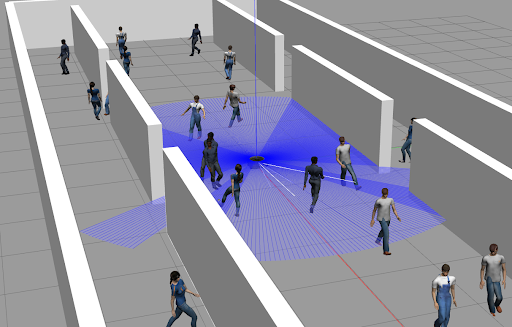
\includegraphics[width=\linewidth]{long_corridor.png}\\
\small Long corridor
\end{minipage}
\hfill
\begin{minipage}{0.32\linewidth}
\centering
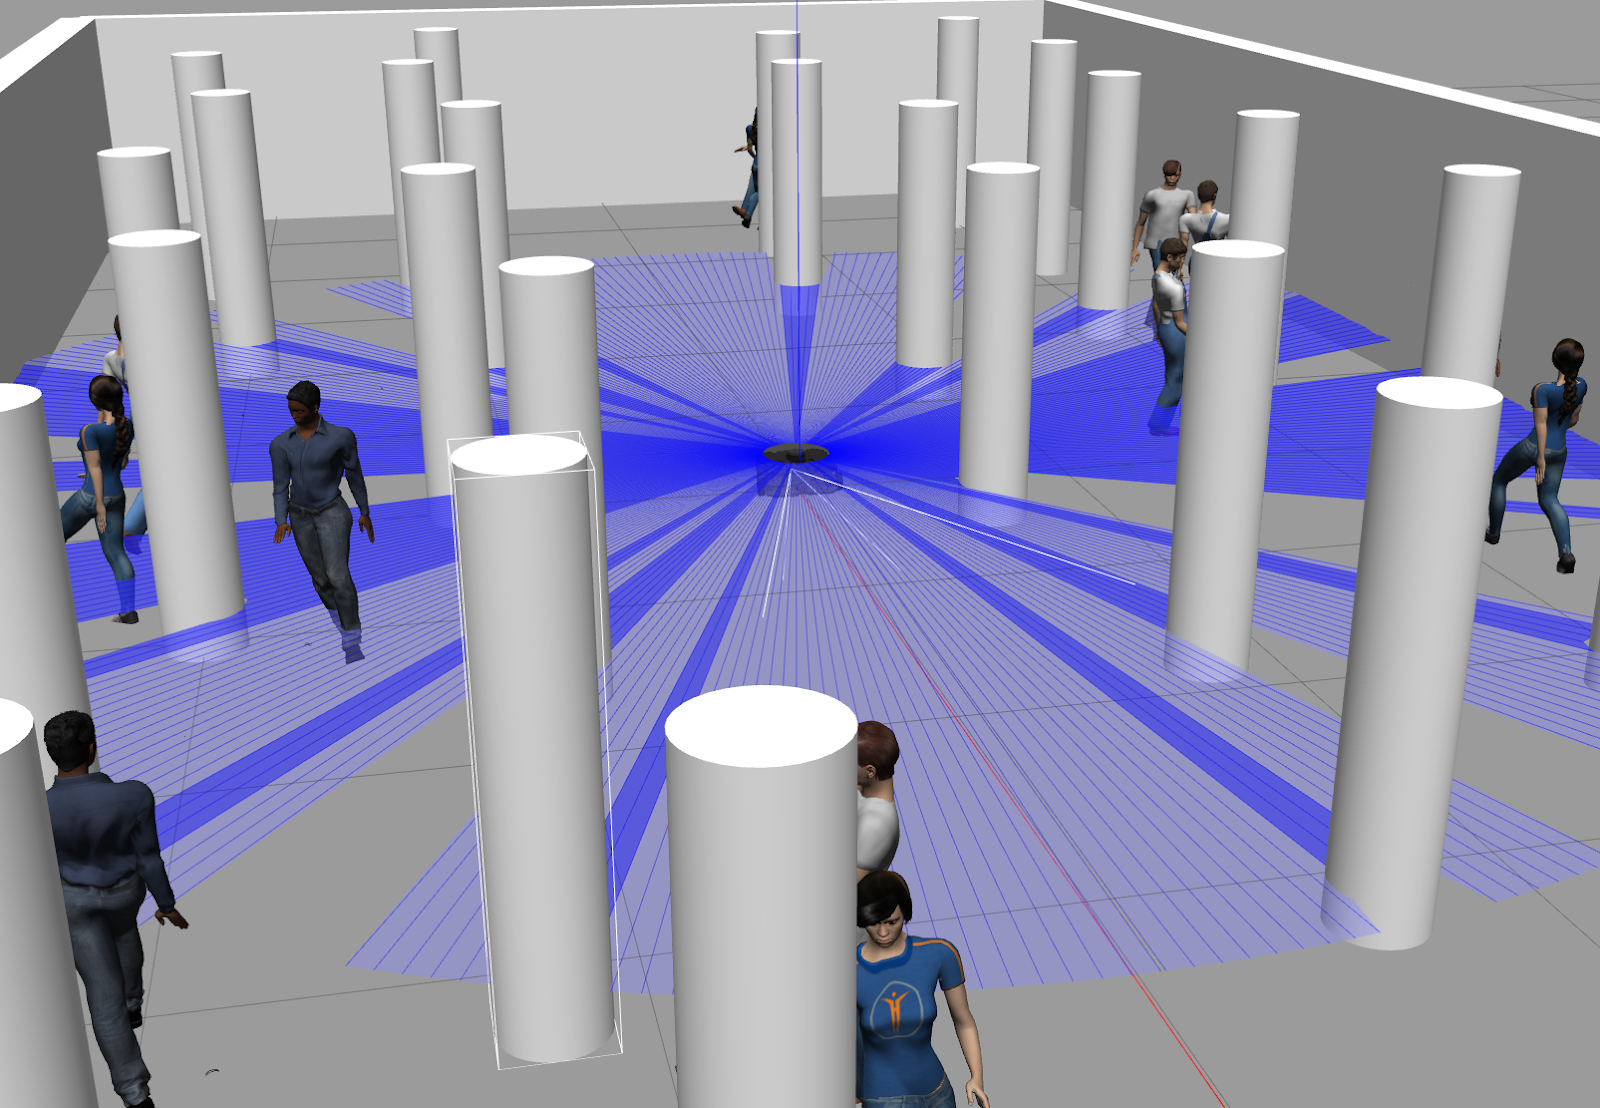
\includegraphics[width=\linewidth]{nonliner_corridor.png}\\
\small Nonlinear corridor
\end{minipage}
\hfill
\begin{minipage}{0.32\linewidth}
\centering
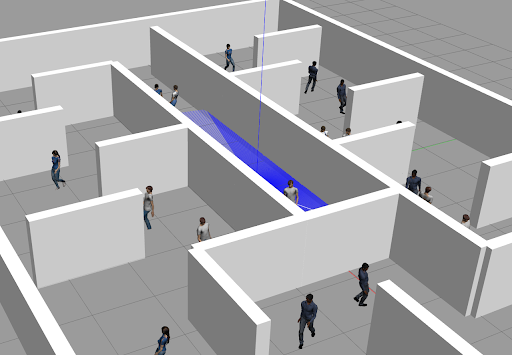
\includegraphics[width=\linewidth]{labyrinth.png}\\
\small Labyrinth
\end{minipage}
\caption{Experimental scene layouts. The long corridor produces many head-on and same-direction pass-by cases; the nonlinear corridor increases the share of smooth turns and local geometry-induced deviations; the labyrinth contains frequent intersections and wall-constrained turns, making the future pedestrian direction less obvious from constant-velocity extrapolation alone.}
\label{fig:three_scenes}
\end{figure}

The long corridor is a narrow passage with bidirectional pedestrian traffic and several side branches; it forces the planner to commit to one side of the corridor before a conflict is fully resolved. The nonlinear corridor adds curved passages and local bends that force pedestrians to deviate from straight-line motion even when not interacting with others, testing the residual model on smoothly nonlinear motion. The labyrinth contains a grid of walls and intersections; the correct future direction is often difficult to infer from a short observation history, which is where the map-aware part of the predictor is most relevant.

All three scenes are evaluated under two interaction modes. \textbf{Mode A} (non-reactive) deliberately makes the benchmark strict: pedestrians follow their waypoints and avoid each other but ignore the robot, so collisions are attributable to the robot's planner. \textbf{Mode B} (reactive) lets pedestrians include the robot in their avoidance field. Mode B is closer to cooperative cohabitation but it also changes the prediction problem: a pedestrian's future depends not only on recent motion, static geometry, and nearby people, but also on the robot's own motion. A predictor trained only on robot-unaware data can fail even if it performs well on ordinary open-loop metrics.

\subsection{Runtime Integration with Nav2 MPPI}

The MPPI algorithm itself is not reimplemented. The experiments use the standard Nav2 MPPI controller and extend it with an additional custom critic, \texttt{PredictedPeopleCritic}, registered as a Nav2 MPPI critic plugin. The predictor is implemented as a separate ROS2 node. It subscribes to the HuNav \texttt{/people} topic, maintains short tracks for observed pedestrians, runs the selected prediction backend, and publishes predicted pedestrian paths as a \texttt{visualization\_msgs/MarkerArray} on \texttt{/predicted\_people\_markers}. The critic subscribes to this topic and adds the dynamic human cost in Eq.~\eqref{eq:human-cost} to each sampled MPPI rollout.

The controller runs at 10~Hz with \texttt{model\_dt}=0.1~s and \texttt{time\_steps}=40 (a 4.0~s rollout horizon). The predictor publishes at 5~Hz. The Kalman backend directly rolls out pedestrian states on the controller time grid with \texttt{pred\_dt}=0.1~s. Learned models use $8$ observations at \texttt{obs\_dt}=0.4~s, matching the training data; the runtime resamples the incoming track history to these observation timestamps by linear interpolation, and if the published prediction is shorter than the MPPI rollout horizon the critic reuses the last available point. Thus, long offline horizons are used for diagnostics, while the runtime integration focuses on the part of the prediction horizon that actually affects the controller.

For each sampled rollout and each controller timestep, the critic compares the sampled robot position with the predicted positions of nearby pedestrians (within a consideration radius, keeping the nearest few per timestep to avoid over-penalizing distant dense crowds). The risk term is Gaussian in distance with a large additional penalty inside the collision radius. The accumulated human cost is time-decayed along the horizon and averaged over MPPI timesteps before being multiplied by the critic weight. The predictor therefore affects MPPI only through this dynamic human cost term; all other Nav2 critics (goal, path-following, static cost map, control constraint) remain unchanged. If a pedestrian disappears, its track is kept for $1.0$~s and then removed; if no valid predictions are available, the critic returns no extra cost.

\subsection{Data Collection and Benchmark Construction}

\textbf{Trajectory logging.} A ROS2 logging node subscribes to the pedestrian state topic and records the 2D position of every simulated agent at a fixed sampling rate. The raw logs are converted into sliding-window prediction cases: an observed pedestrian trajectory, neighboring pedestrian context, and a ground-truth future. The common observation setting is $8$ observed positions with $\Delta t=0.4$~s (3.2~s history). Future trajectories are stored for two horizons: 12 steps for the navigation-facing predictor and 26 steps for longer offline diagnostics. The full offline benchmark contains approximately $30{,}000$ trajectory snippets across all three scenes after filtering. A fixed held-out evaluation subset of $2{,}144$ cases is used for the non-reactive prediction benchmark.

\textbf{Dataset split and leakage control.} Data is not generated by replaying the same fixed benchmark episodes used for closed-loop evaluation. Instead, logs are recorded by manually driving the robot through handwritten routes while $20$ simulated pedestrians follow HuNav behaviors; about one hour of simulation time is used for the robot-aware collection. The split is performed at the log/trajectory block level rather than by independently shuffling windows. For the final robot-reactive predictor experiments, the long-corridor holdout uses the last 25\% temporal block, while earlier blocks and the additional scenes are used for training and curation. Windows with invalid tracks, insufficient length, or uninformative stationary-robot segments are removed.

\textbf{Robot-aware curated dataset.} To study why predictors trained without robot influence do not transfer reliably to robot-reactive navigation, an additional curated dataset is constructed from runs in which pedestrians react to the robot. The selected robot influence force is $0.75$, the most informative setting in the force sweep (Section~\ref{sec:force-sweep}): it creates visible robot-induced avoidance and non-linear local motion, but the robot still encounters pedestrians often enough for the planner to be meaningfully tested. The curated data is built from the same three scene families and keeps only pedestrians within a $6$~m radius of the robot, because these are the trajectories that can affect the local planner. The dataset generation uses a $2$~m neighbor radius, up to $16$ neighbors, and a stride of $5$ frames between candidate windows. Candidate windows in which the robot is stationary for the full observation and prediction window are removed, so the learned correction is trained on windows in which the robot is moving or begins moving during the episode. The resulting curated set contains approximately $13{,}600$ training cases and $4{,}600$ test cases, with scene diversity preserved so that the model does not overfit to a single corridor geometry. Each case uses $8$ observed positions with $\Delta t=0.4$~s, corresponding to a $3.2$~s observation window; the model predicts $12$ future steps for navigation (sufficient for the local MPPI controller), and $26$-step horizons are also retained for offline diagnostics.

The curated dataset is stratified by motion type in order to understand how robot influence changes the distribution of training examples. The classification is not used as a direct training label for the residual model. Instead, it is used for analysis, balancing, and interpretation of the force-sweep results. For an observation window $\{\mathbf{p}_t\}_{t=1}^{8}$, define
\[
L=\sum_{t=2}^{8}\|\mathbf{p}_{t}-\mathbf{p}_{t-1}\|_2,
\qquad
D=\|\mathbf{p}_{8}-\mathbf{p}_{1}\|_2,
\qquad
\Delta\phi_{\deg}=\tfrac{180}{\pi}\sum_{t=3}^{8}|\operatorname{wrap}(\phi_t-\phi_{t-1})|.
\]
Linear and turning classes are defined by $\Delta\phi_{\deg}<30^\circ$ and $\Delta\phi_{\deg}\ge 45^\circ$. Stop-go cases satisfy $\max_t v_t\ge 0.25$, $\min_t v_t\le 0.10$, and $\max_t v_t-\min_t v_t\ge 0.25$. Interaction cases satisfy $1\le N_{\text{neigh}}\le 3$ and $d_{\min}\le 1.5$~m; dense interaction cases satisfy $N_{\text{neigh}}\ge 4$ and $d_{\min}\le 1.5$~m. Complex cases activate at least two of these indicators.

\begin{figure}[H]
\centering
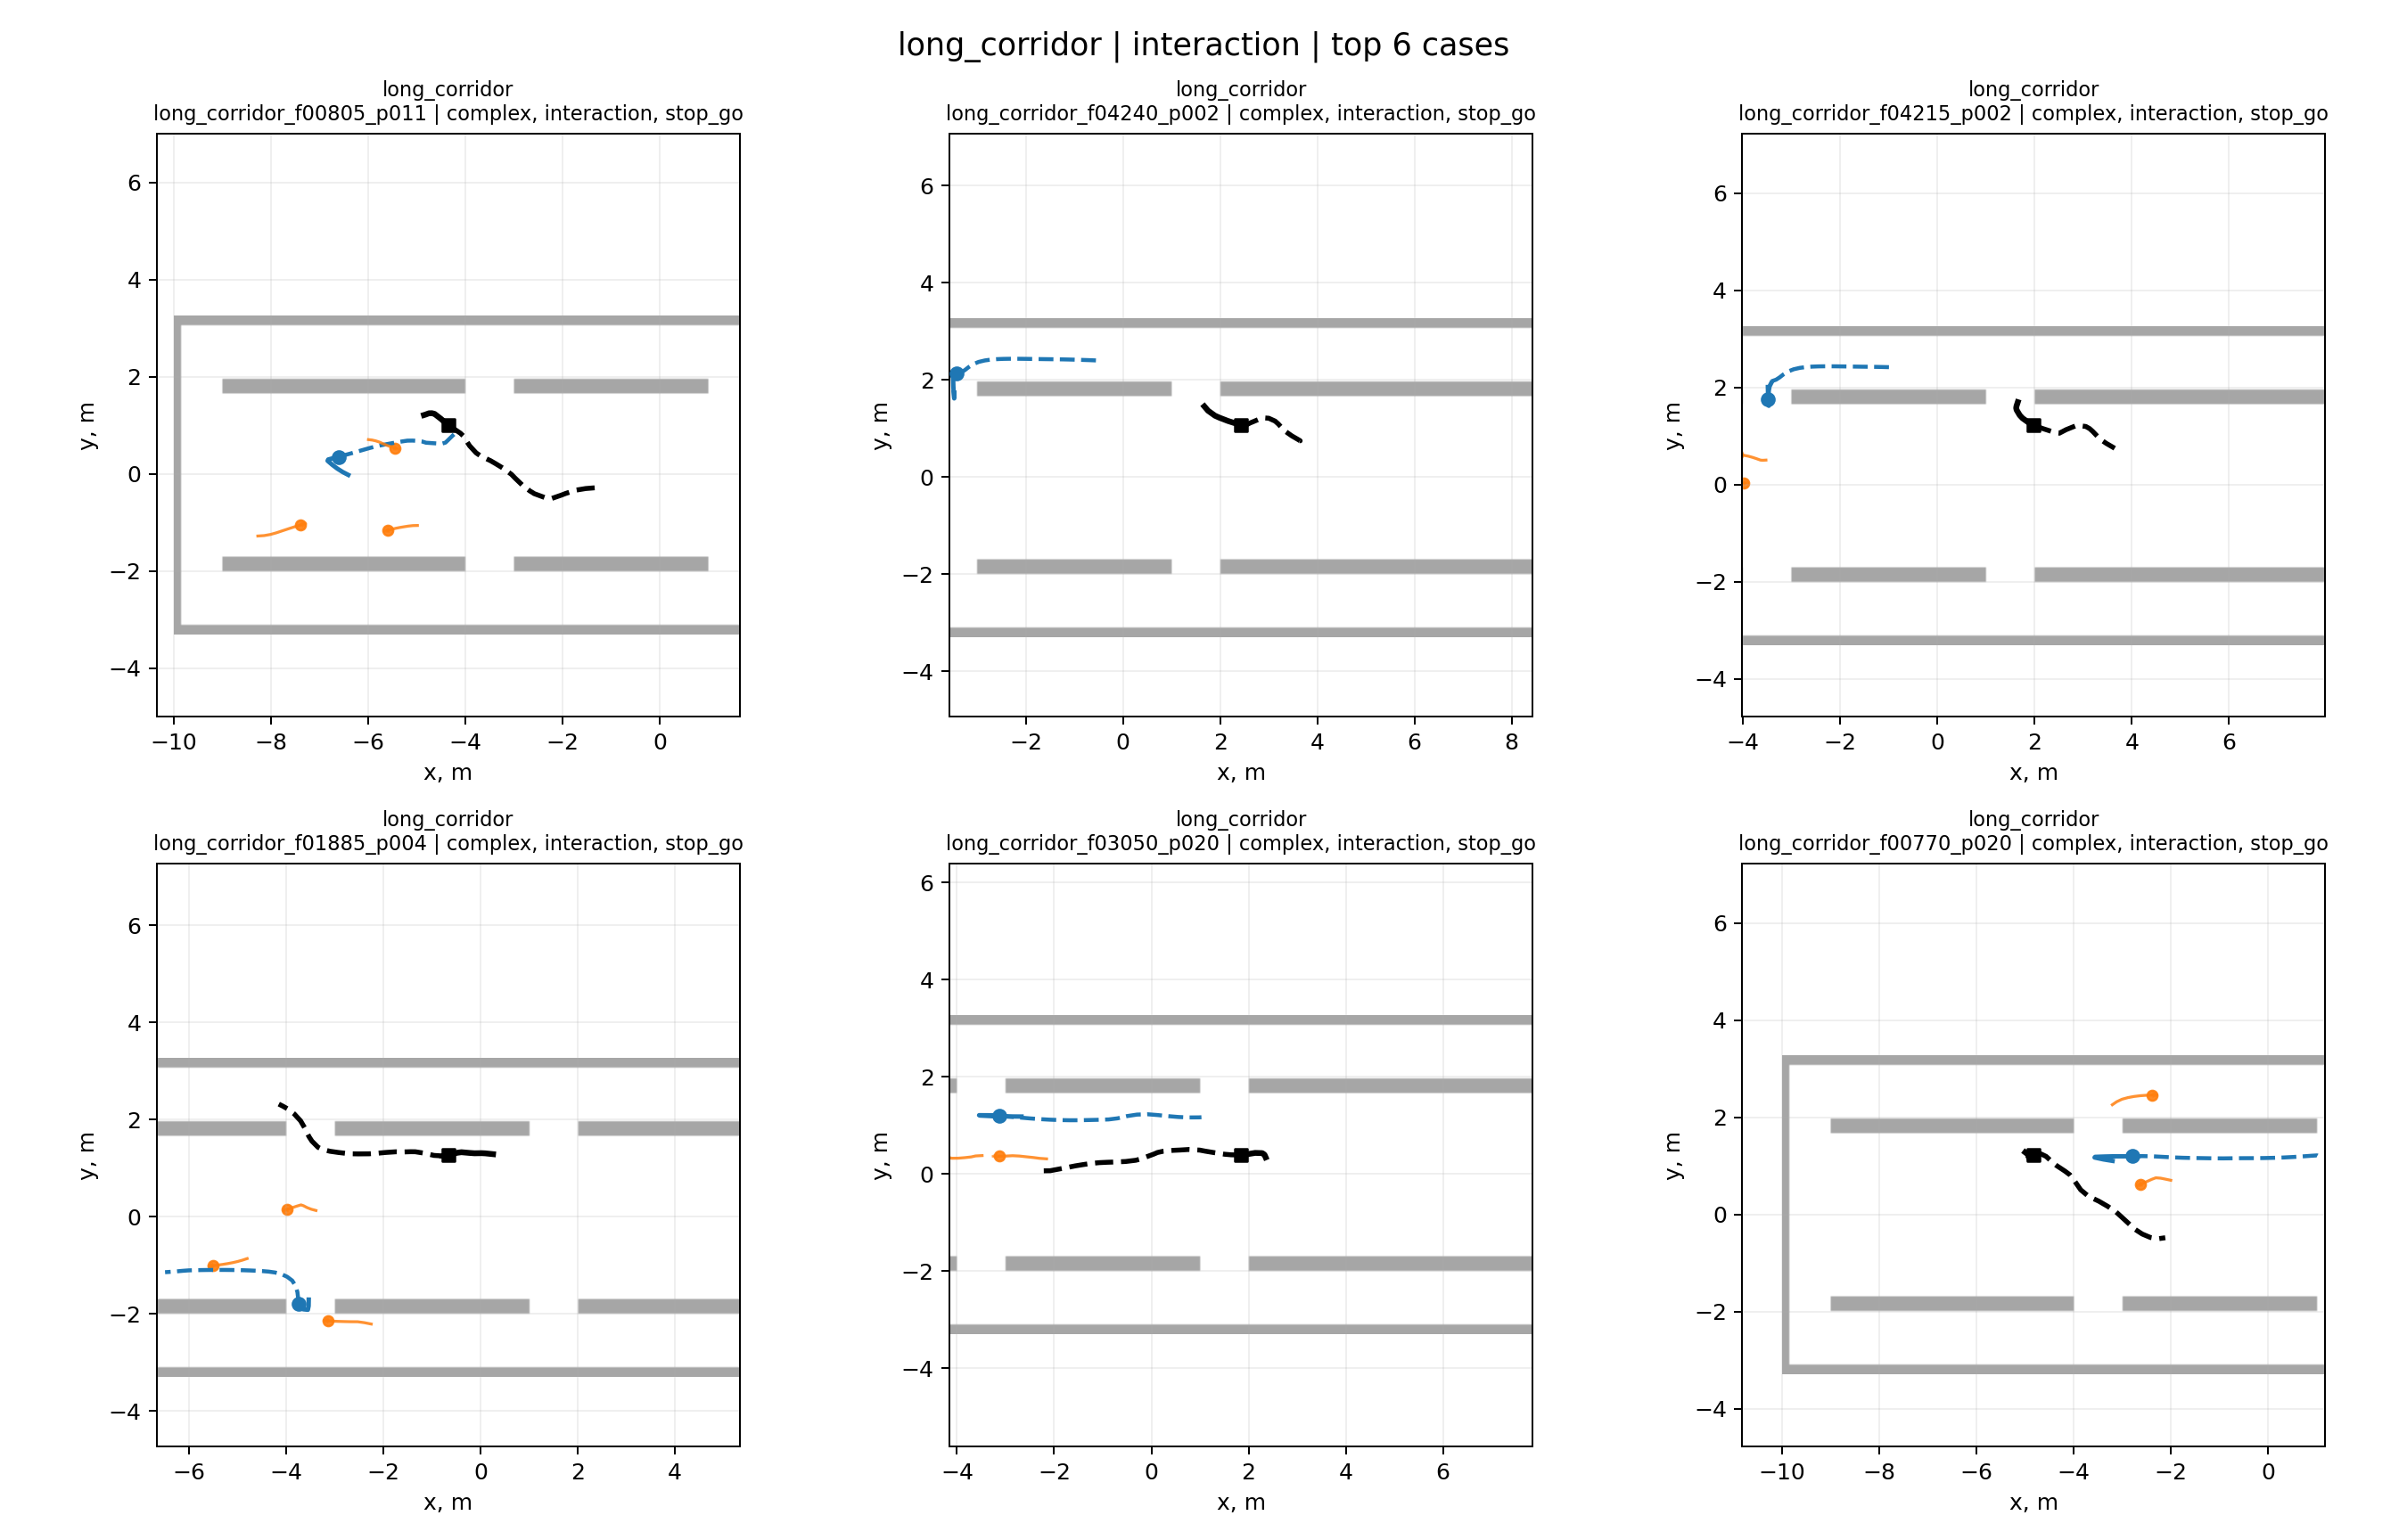
\includegraphics[width=0.92\linewidth]{dataset_long_corridor_interaction.png}
\caption{Interaction cases from the curated long-corridor dataset. Black marks the robot, blue marks the target pedestrian, and remaining colored points are other nearby pedestrians.}
\label{fig:dataset_interaction}
\end{figure}

\begin{figure}[H]
\centering
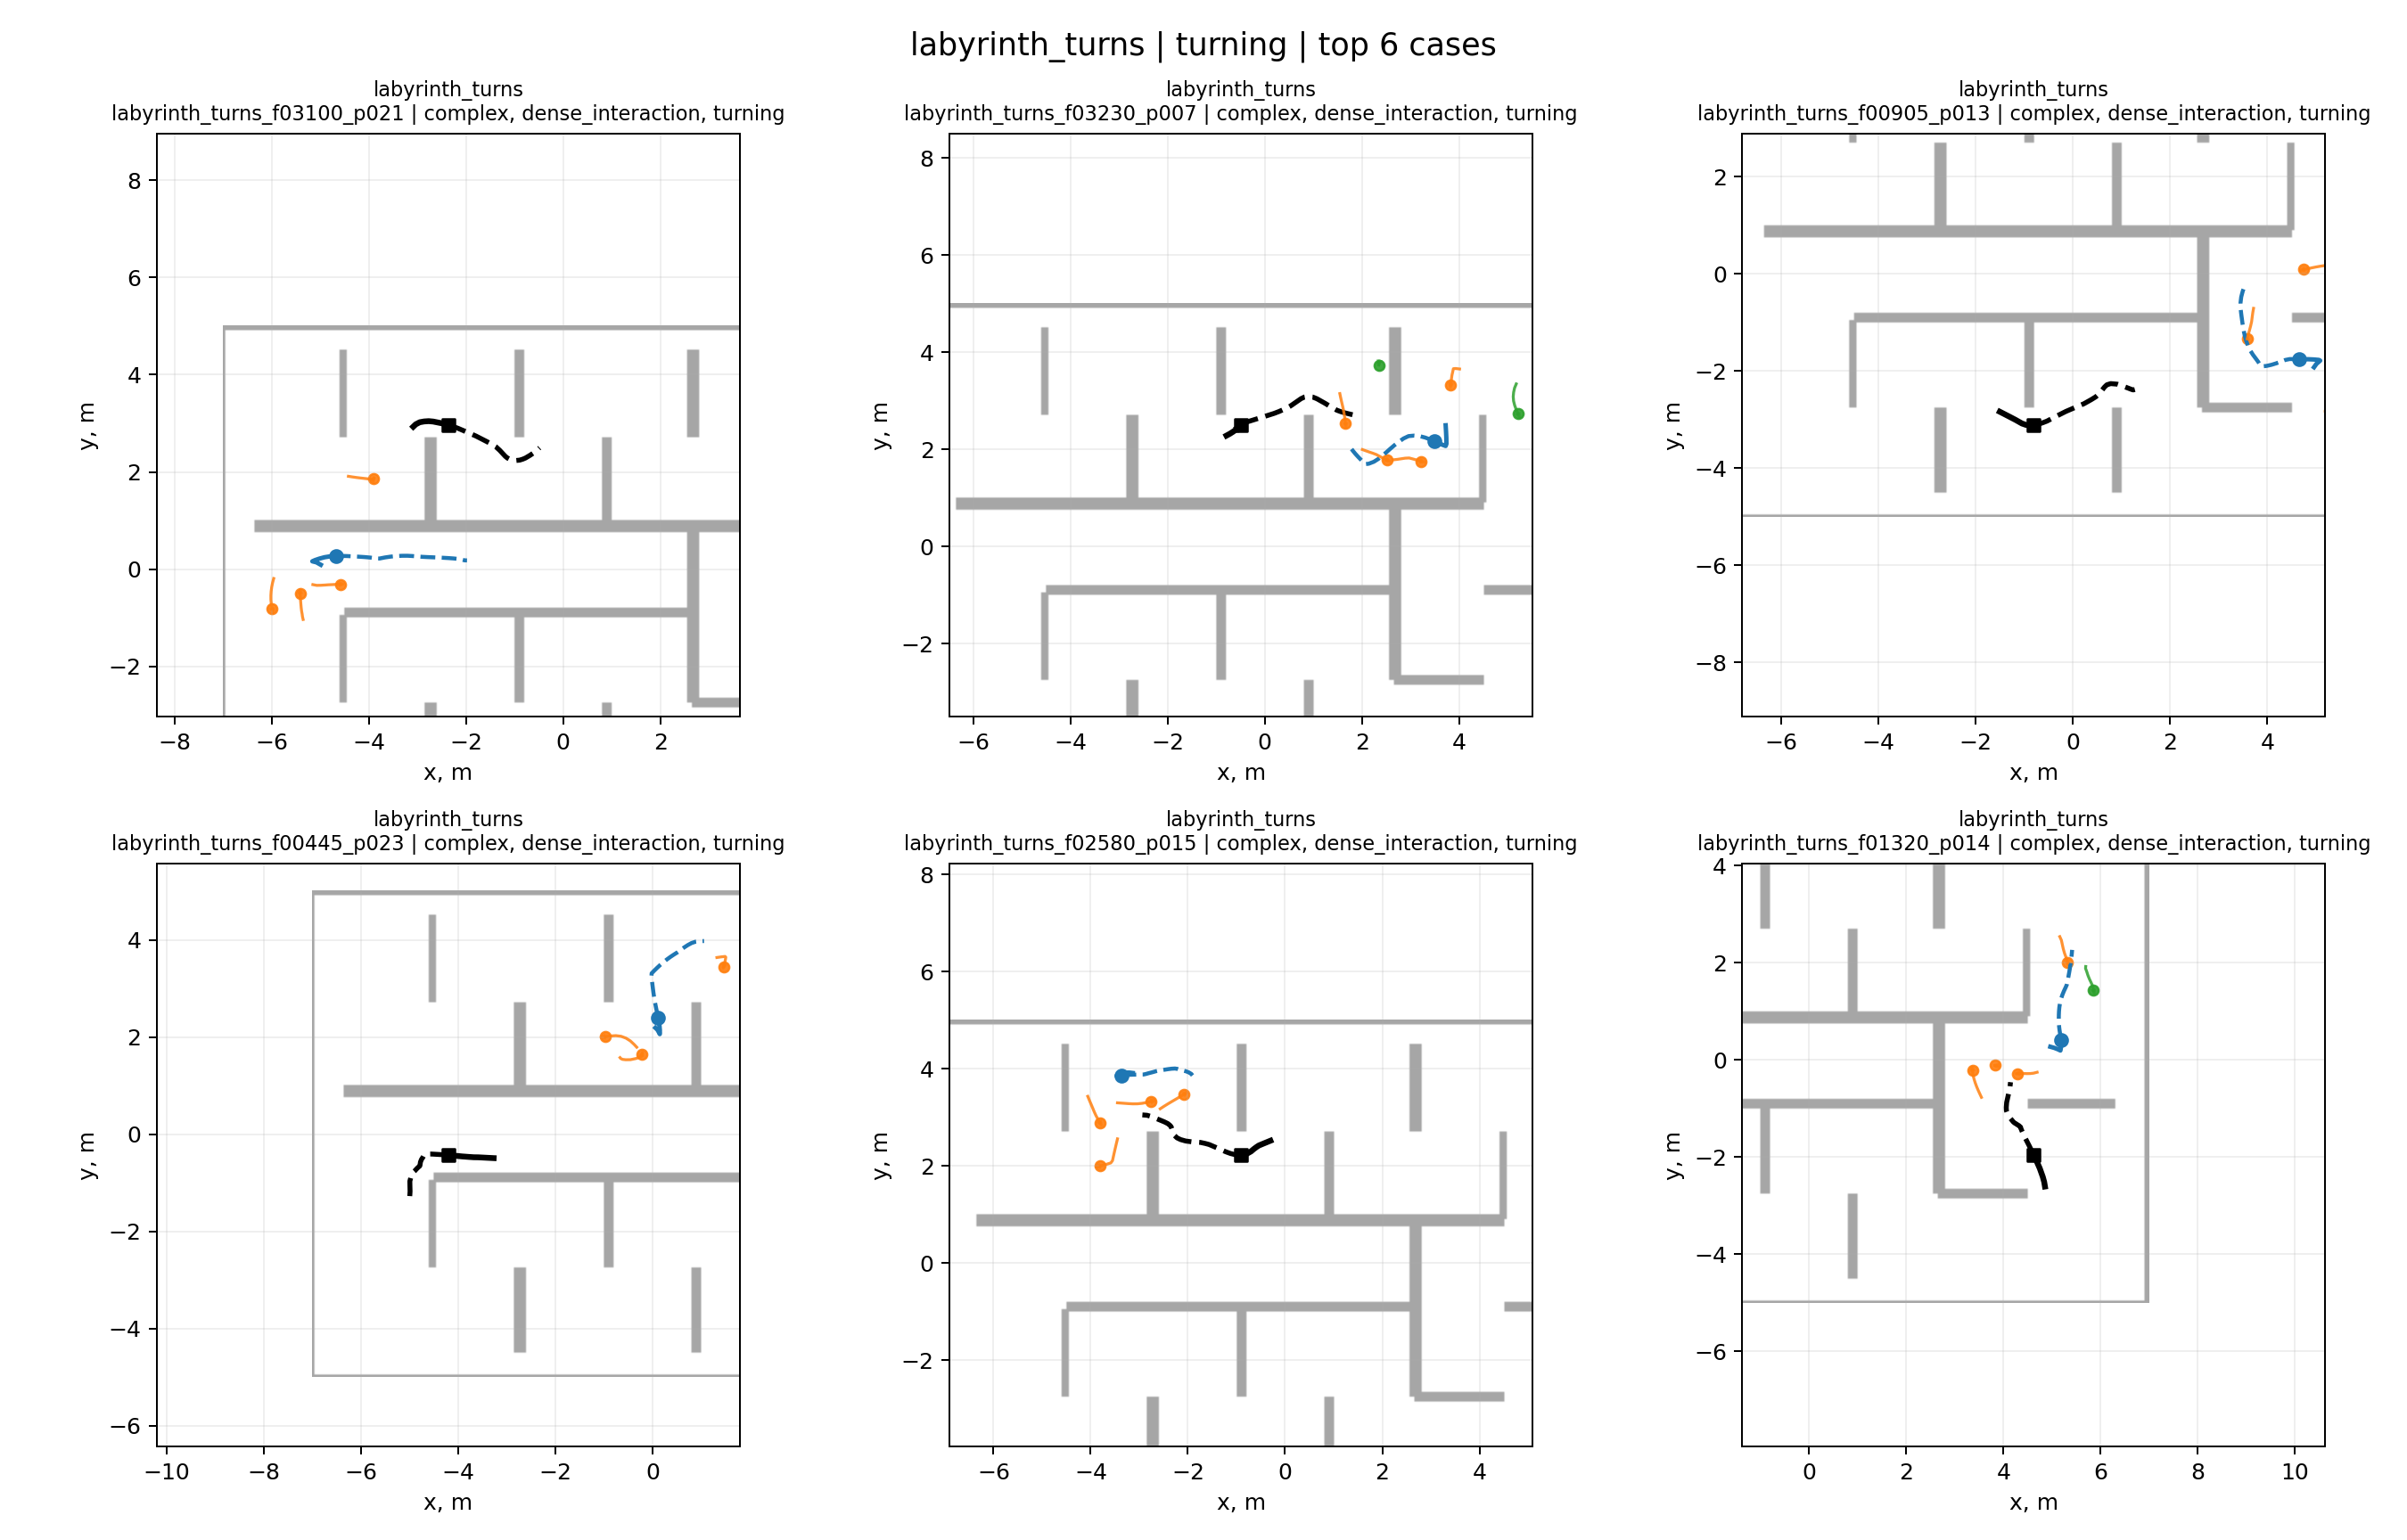
\includegraphics[width=0.92\linewidth]{dataset_labyrinth_turning.png}
\caption{Turning cases from the curated labyrinth dataset. The labyrinth geometry creates turns near walls and intersections, where a constant-velocity Kalman forecast is likely to continue through the wall or miss the future direction change.}
\label{fig:dataset_turning}
\end{figure}

\subsection{Metrics and Navigation Protocol}

Three groups of metrics are used.

\emph{Offline prediction metrics:}
\begin{itemize}[leftmargin=2em,itemsep=2pt,topsep=2pt]
\item \textbf{Average Displacement Error (ADE).} Mean Euclidean distance, in meters, between predicted and ground-truth positions averaged over all $H$ future steps. Lower is better.
\item \textbf{Final Displacement Error (FDE).} Euclidean distance between predicted and ground-truth positions at the final horizon step $H$, in meters. Lower is better.
\end{itemize}
Both are reported at $H=12$ (navigation-facing horizon) and at $H=26$ (longer offline diagnostic horizon).

\emph{Streaming stability metrics} (defined formally in Section~\ref{sec:stabilization}, all measured under the same observation stream used at runtime):
\begin{itemize}[leftmargin=2em,itemsep=2pt,topsep=2pt]
\item \textbf{Inter-query jitter.} Mean position difference between two predictions of the same absolute future time produced at two consecutive planner ticks; measures how much the cost field of Eq.~\eqref{eq:human-cost} moves between control cycles.
\item \textbf{Prediction jerk.} Mean Euclidean norm of the third time-derivative of the predicted trajectory; measures the smoothness of a single forecast over the horizon.
\item \textbf{Acceleration error.} Mean error between predicted and ground-truth accelerations along the prediction; captures dynamic plausibility of the forecast.
\item \textbf{Residual norm} and \textbf{predicted acceleration energy.} Diagnostic quantities reported for the residual predictor, used during checkpoint selection.
\end{itemize}

\emph{Closed-loop navigation metrics} (computed over a full navigation episode):
\begin{itemize}[leftmargin=2em,itemsep=2pt,topsep=2pt]
\item \textbf{Time to goal.} Wall-clock seconds from start to goal achievement. Lower is better.
\item \textbf{Path length.} Total length, in meters, of the executed robot trajectory. Lower is better.
\item \textbf{Minimum distance to pedestrians.} Smallest robot--human distance encountered during the episode. Higher is better.
\item \textbf{Average distance to pedestrians.} Mean robot--human distance to the nearest pedestrian over the episode. Higher is better.
\item \textbf{Collision count.} Number of collision events during the episode. Lower is better.
\item \textbf{Constraint violation time.} Cumulative time, in seconds, during which the robot is closer than the personal-space radius to any pedestrian. Lower is better.
\item \textbf{Robot influence (diagnostic).} A measure of how much pedestrian motion is altered by the robot's presence; reported only to characterize the interaction regime, not to compare predictors.
\end{itemize}

Each navigation trial executes a fixed route through the scene while the crowd follows the configured behavior mode. Whenever predictors are compared directly, paired evaluation is used: each algorithm is run on the same initial conditions and route sequence so that metric differences reflect the predictor rather than random variation. Statistical comparisons use the paired Wilcoxon signed-rank test.

% ============================================================
%  5. RESULTS
% ============================================================
\section{Results}
\label{sec:results}

The results are organized from open-loop to closed-loop: the offline prediction benchmark (\ref{sec:res-offline}), the robot influence sweep that motivates the reactive dataset (\ref{sec:force-sweep}), the reactive predictor benchmark with streaming stability metrics (\ref{sec:res-reactive-pred}), compute footprint (\ref{sec:res-compute}), and finally paired closed-loop navigation comparisons in Mode~A and Mode~B (\ref{sec:res-nav}).

\subsection{Offline Prediction Benchmark}
\label{sec:res-offline}

Table~\ref{tab:offline} presents the offline prediction results on the $2{,}144$-case evaluation subset.

\begin{table}[H]
\centering
\caption{Offline prediction metrics on the evaluation subset ($N=2{,}144$ trajectories, three scenes combined). ADE and FDE are measured in meters at prediction horizons $H=12$ and $H=26$; lower is better.}
\label{tab:offline}
\resizebox{\textwidth}{!}{%
\begin{tabular}{lcccc}
\toprule
\textbf{Model} & \textbf{ADE@12 $\downarrow$} & \textbf{FDE@12 $\downarrow$} & \textbf{ADE@26 $\downarrow$} & \textbf{FDE@26 $\downarrow$} \\
\midrule
Kalman Filter & 0.117 & 0.228 & 0.284 & 0.620 \\
Social GRU & 0.279 & 0.588 & 0.720 & 1.597 \\
SocialVAE (pre-trained) & 0.211 & 0.489 & 0.595 & 1.314 \\
Kalman + Residual (naive) & \textbf{0.084} & \textbf{0.172} & \textbf{0.219} & \textbf{0.487} \\
Kalman + Gated Residual (stabilized) & 0.113 & 0.220 & 0.275 & 0.599 \\
\bottomrule
\end{tabular}
}
\end{table}

Several observations follow. First, the Kalman filter substantially outperforms both Social GRU and the pre-trained SocialVAE on all metrics. Both learned baselines were trained on real outdoor pedestrian datasets (Social GRU on Trajectron++~[3] preprocessed ETH/UCY, SocialVAE on the HOTEL scene of ETH/UCY) and therefore suffer from a substantial domain-shift penalty when evaluated on the simulated indoor scenes used here; the gap is especially large for Social GRU, which has neither pre-trained encoder weights nor a stochastic decoder to absorb mismatched trajectory distributions. Second, the naive residual achieves the best offline scores by a substantial margin, confirming that the correction network learns to address the Kalman filter's systematic errors. Third, the stabilized gated residual sacrifices a small amount of offline accuracy relative to the naive residual, because the gate suppresses the correction on straight segments, but this is the deliberate trade-off for online stability. The improvement of the naive residual over Kalman is larger on the labyrinth and nonlinear-corridor subsets than on the long corridor; the cost-map branch contributes to this gain on turns and near obstacles, though its effect on aggregate metrics is modest because the benchmark is dominated by approximately linear corridor trajectories.

\subsection{Robot Influence Sweep and Distribution Shift}
\label{sec:force-sweep}

Before training a robot-aware residual predictor, the effect of the HuNav \texttt{robot\_force\_scale} is evaluated using the Kalman baseline. If humans are configured to ignore the robot, the value is forced to $0.0$. A value of $1.0$ enables the full configured robot social-force channel; values above $1.0$ amplify robot-induced avoidance. The force is swept and each setting is evaluated over four episodes.

\begin{figure}[H]
\centering
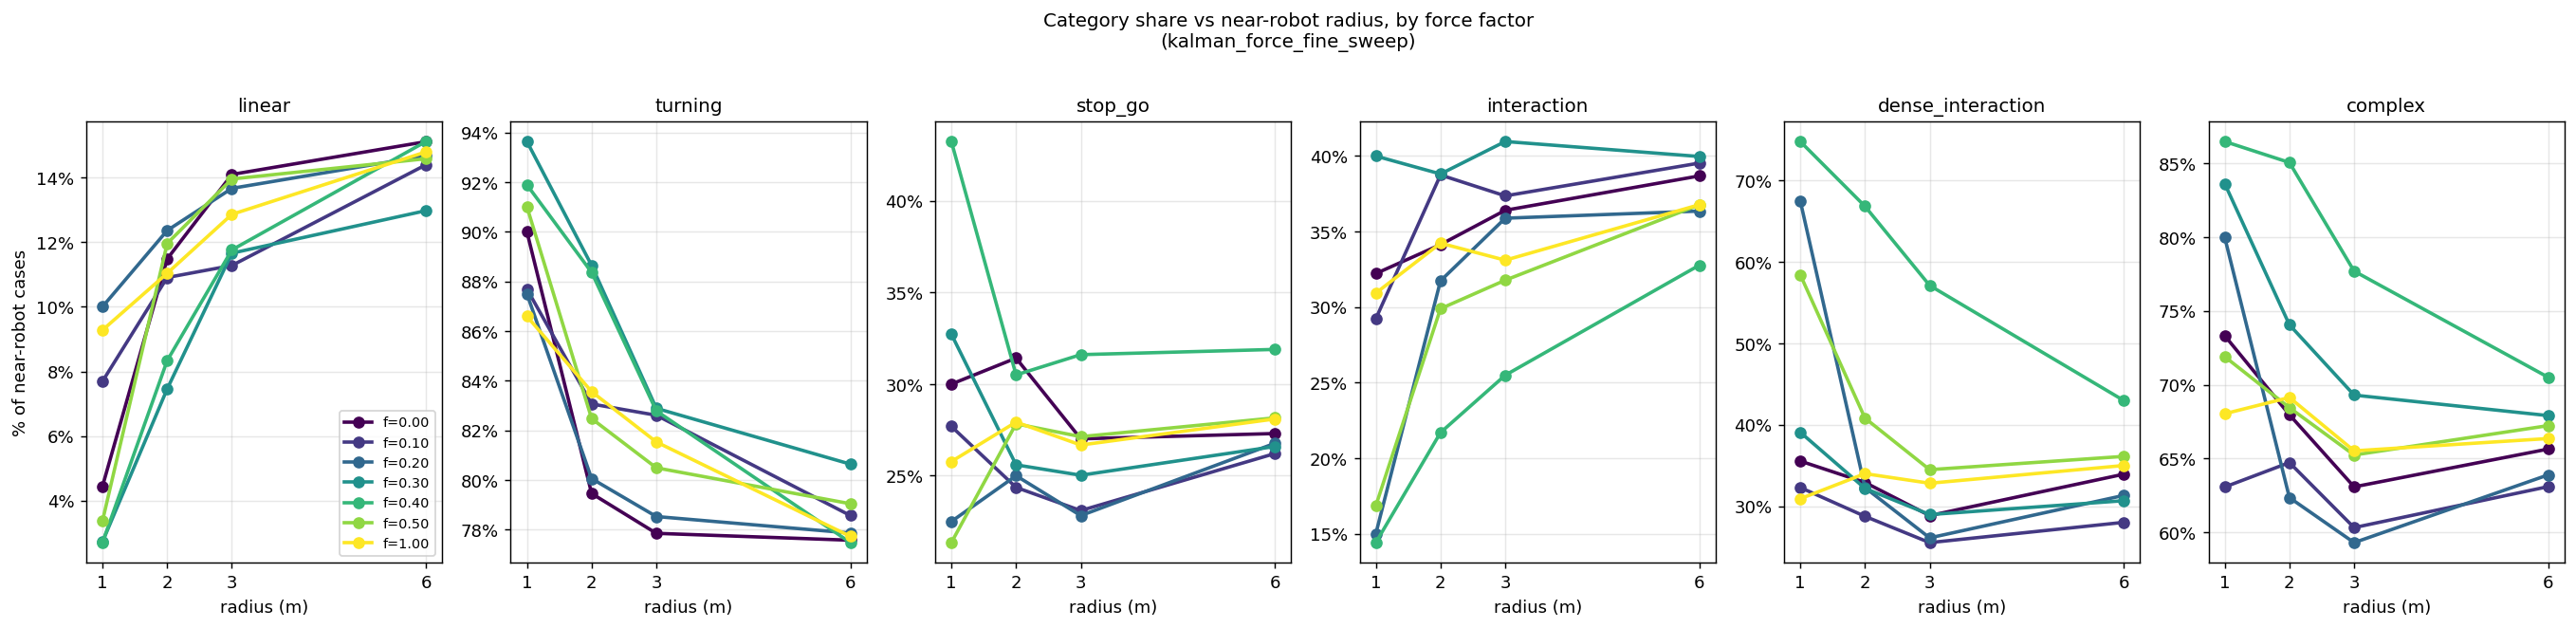
\includegraphics[width=0.95\linewidth]{category_vs_radius_by_force.png}
\caption{Motion category distribution as a function of distance to the robot and robot influence force. As force increases, local behavior near the robot contains more turns and complex interactions, while some direct close interactions decrease because pedestrians avoid the robot earlier.}
\label{fig:category_force}
\end{figure}

\begin{figure}[H]
\centering
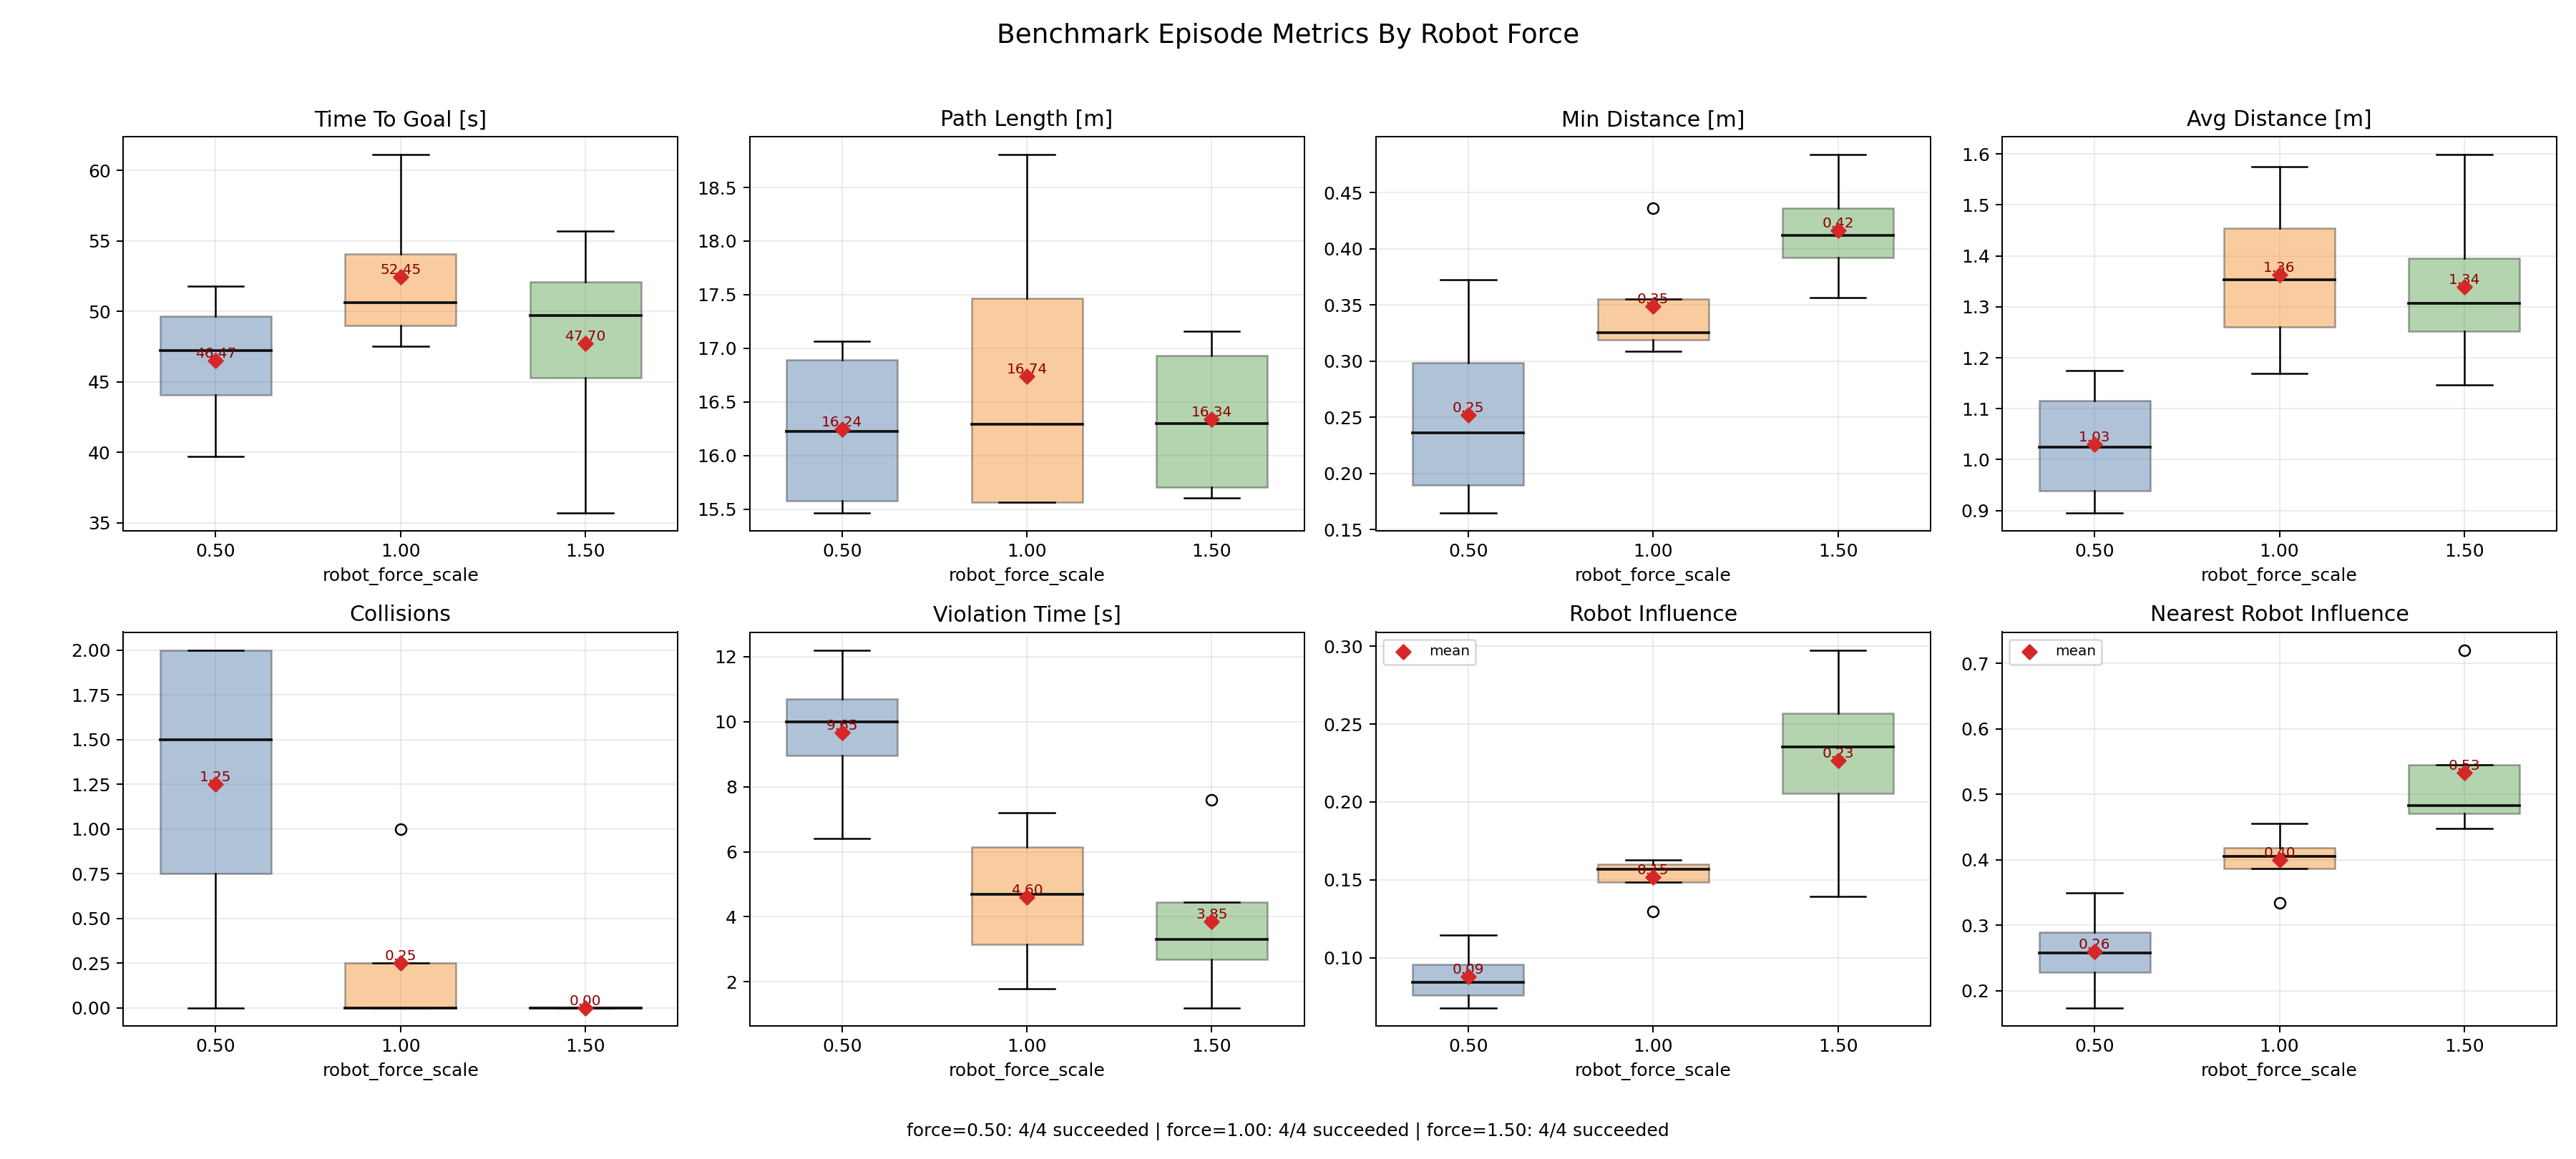
\includegraphics[width=0.95\linewidth]{benchmark_metrics_boxplot_force0p75.png}
\caption{Navigation metrics for the Kalman baseline under different robot influence force values. Robot influence is diagnostic and measures how strongly pedestrian motion is affected by the robot. The force-$0.75$ setting is selected for data collection: it produces a clear robot-reactive distribution shift while preserving enough close interactions for the planner and predictor to be tested.}
\label{fig:force_metrics}
\end{figure}

At force $0$, pedestrians do not react to the robot (the non-reactive setting). At force $2$, pedestrians avoid the robot so aggressively that collisions nearly disappear and the benchmark becomes uninformative for measuring planner improvement. Force $0.75$ is therefore used for new logs and model training: it is difficult enough that close encounters and collisions remain available for learning, but it is clearly different from the non-reactive case.

Figure~\ref{fig:category_force} gives the main explanation for the transfer problem. As the robot influences pedestrians, purely linear cases become less representative near the robot, while turning, dense-interaction, and complex cases occupy a larger share of the local dataset. At a distance of about $3$~m, the local pedestrian behavior is already drawn from a different distribution than in the non-reactive dataset. This is why a predictor trained only on non-reactive data does not transfer cleanly to reactive navigation.

\subsection{Reactive Predictor Benchmark with Stability Metrics}
\label{sec:res-reactive-pred}

Learned predictors are evaluated on force-$0.75$ long-corridor holdout windows with $N=25{,}000$ sampled cases and horizon $H=12$. Two model families are compared: the Kalman-residual MLP trained on robot-aware logs from the three scenes, and SocialVAE fine-tuned on the same data. The SocialVAE fine-tuning is intentionally limited: the pre-trained checkpoint is used as initialization, the encoder and latent layers are frozen, and only the decoder head (\texttt{rnn\_fy\_init} and \texttt{dec}) is trained. This yields $\approx 271$k trainable parameters versus $\approx 131$k for the residual MLP. The standard fine-tuning loss is $\mathcal{L}_{\mathrm{VAE}}=\mathcal{L}_{\mathrm{rec}}+0.2\,\mathcal{L}_{\mathrm{KL}}$; a stable variant adds $0.2\,\mathcal{L}_{\mathrm{vel}}+0.05\,\mathcal{L}_{\mathrm{jerk}}$.

All learned predictors use the same local trajectory normalization: the target pedestrian's last observed position is the local origin, and the local $x$-axis is aligned with recent velocity when well-defined. Observed target motion, neighbor trajectories, the Kalman forecast, and the residual target are represented in this local frame. The residual model predicts the difference between ground-truth and Kalman futures; the map branch receives a normalized $32\times 32$ local cost-map patch covering a $6$~m square around the target. The same normalization is used at inference.

\begin{figure}[H]
\centering
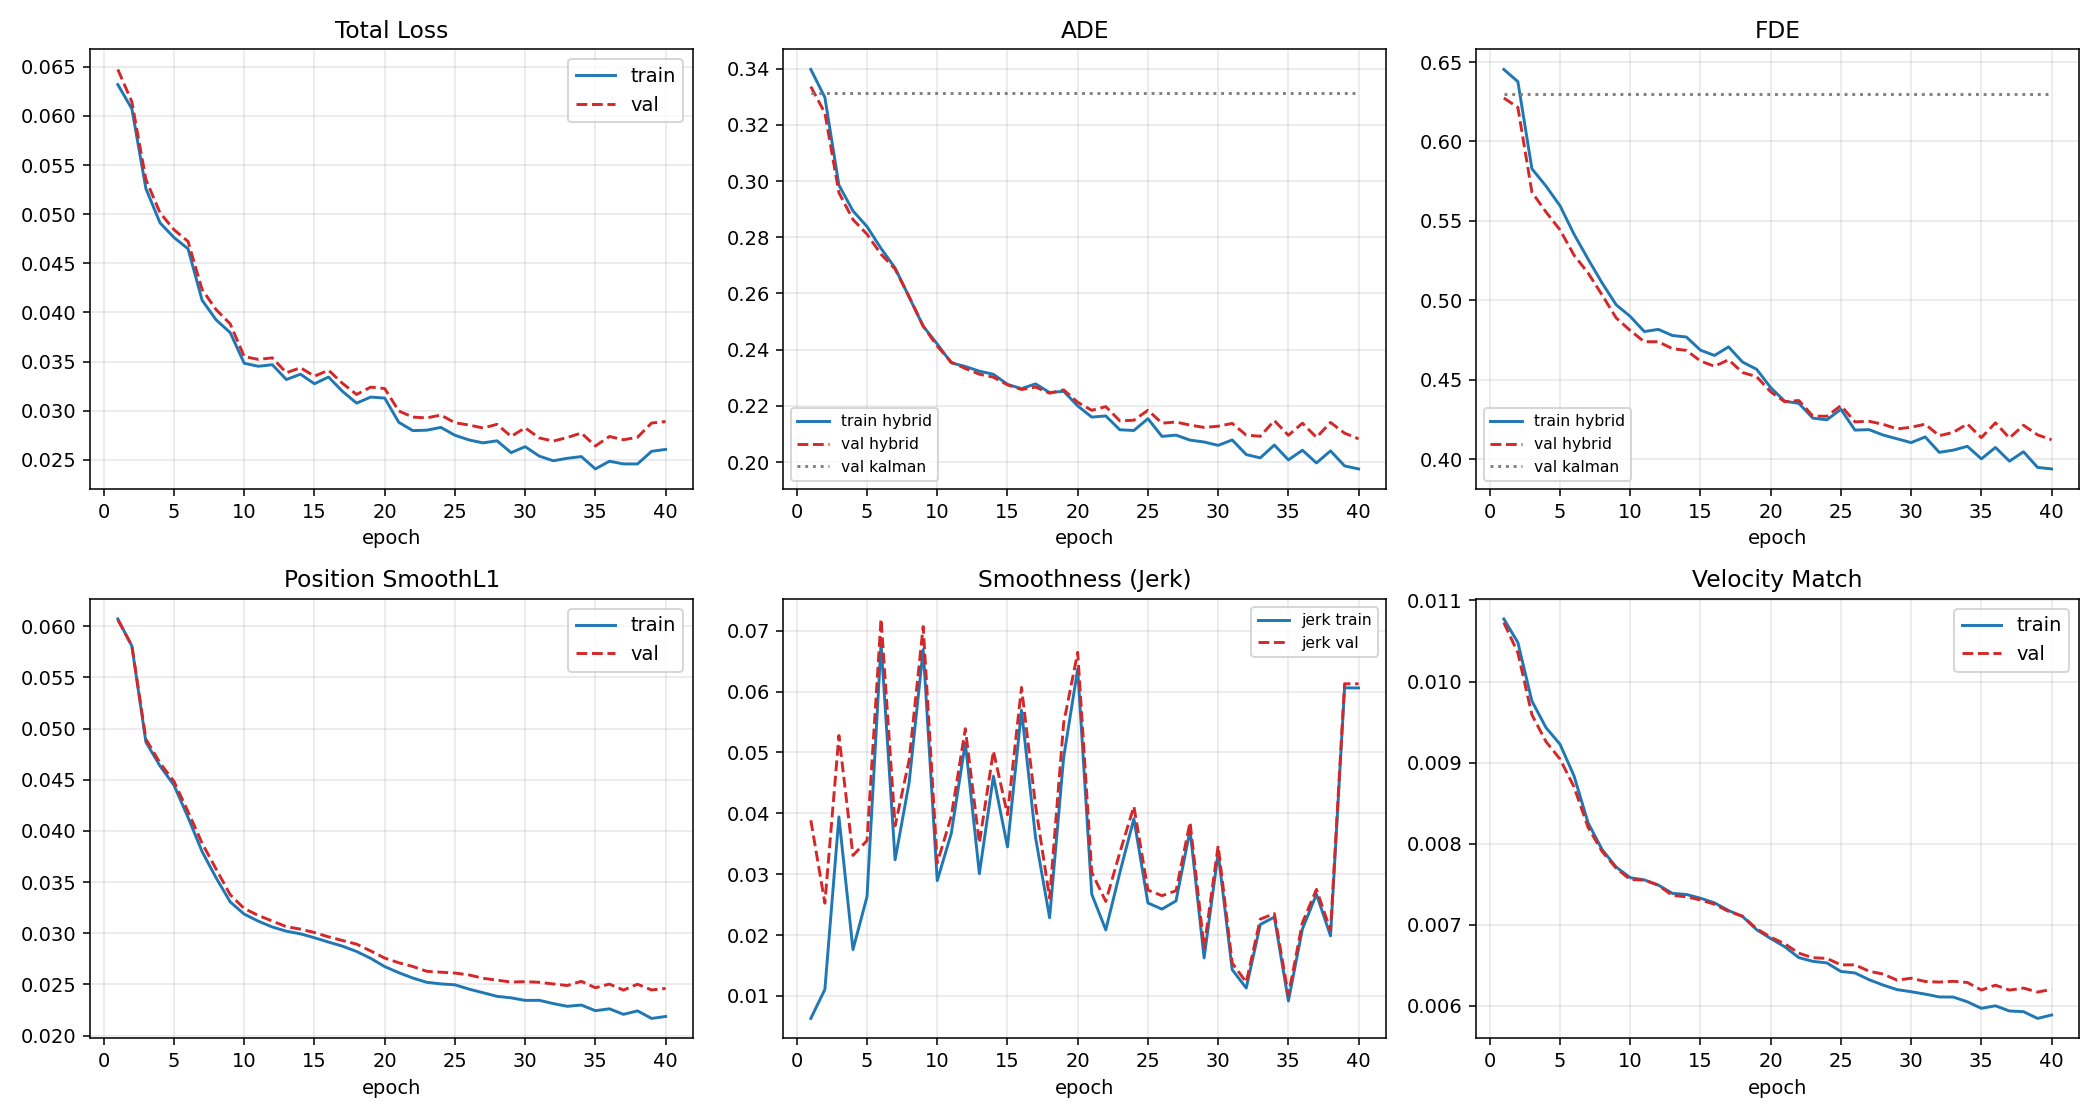
\includegraphics[width=0.82\linewidth]{residual_force0p3_loss.png}
\caption{Training curves for the Kalman-residual MLP. The best-ADE checkpoint is not always the best navigation checkpoint: prediction jerk and residual magnitude must also be controlled, as shown in Table~\ref{tab:reactive_predictor_sweep}.}
\label{fig:residual_force_loss}
\end{figure}

\begin{table}[H]
\centering
\scriptsize
\caption{Reactive long-corridor predictor sweep on force-$0.75$ data, $N=25{,}000$, $H=12$. ADE/FDE are spatial errors in meters; \texttt{pred\_acc}, \texttt{pred\_jerk}, and \texttt{jitter} measure temporal stability under streaming evaluation; lower is better in all columns. A $\star$ marks the row selected as the navigation predictor (Configuration~B).}
\label{tab:reactive_predictor_sweep}
\resizebox{\textwidth}{!}{%
\begin{tabular}{lccccccc}
\toprule
\textbf{Model / setup} & \textbf{ADE $\downarrow$} & \textbf{FDE $\downarrow$} & \textbf{pred\_acc $\downarrow$} & \textbf{acc\_err $\downarrow$} & \textbf{pred\_jerk $\downarrow$} & \textbf{jitter $\downarrow$} & \textbf{res\_norm $\downarrow$} \\
\midrule
Kalman & 0.262 & 0.529 & \textbf{0.0000} & \textbf{0.0614} & \textbf{0.0000} & 0.0754 & -- \\
SocialVAE & \textbf{0.169} & 0.384 & 0.0197 & 0.0651 & 0.0318 & 0.0738 & 0.1771 \\
SocialVAE stable & 0.171 & 0.387 & 0.0188 & 0.0642 & 0.0221 & 0.0735 & 0.1795 \\
Residual old, $\alpha=0.8$, no gate & 0.175 & \textbf{0.360} & 0.0375 & 0.0770 & 0.1560 & 0.0668 & 0.1556 \\
Residual stable-select, $\alpha=0.8$, no gate & 0.176 & 0.361 & 0.0261 & 0.0691 & 0.0860 & 0.0641 & 0.1668 \\
Residual smooth e70 stable, $\alpha=0.8$, no gate & 0.192 & 0.393 & 0.0242 & 0.0672 & 0.0493 & \textbf{0.0623} & 0.1524 \\
Residual smooth e70 bestADE, $\alpha=0.8$, no gate & 0.186 & 0.374 & 0.0231 & 0.0669 & 0.0539 & 0.0631 & 0.1643 \\
$\star$ Residual smooth e70 bestADE, $\alpha=0.8$, soft gate & 0.197 & 0.404 & 0.0119 & 0.0629 & 0.0285 & 0.0685 & 0.1009 \\
Residual smooth e70 bestADE, $\alpha=0.8$, $\beta_s=0.3$, no gate & 0.183 & 0.368 & 0.0239 & 0.0673 & 0.0567 & 0.0641 & 0.1686 \\
Residual smooth e70 bestADE, $\alpha=0.8$, $\beta_s=0.3$, soft gate & 0.194 & 0.399 & 0.0124 & 0.0631 & 0.0303 & 0.0698 & 0.1036 \\
Residual smooth e70 bestADE, $\alpha=0.8$, clip 0.25, soft gate & 0.214 & 0.450 & 0.0153 & 0.0661 & 0.0430 & 0.0720 & 0.0757 \\
Residual smooth e70 bestADE, $\alpha=0.7$, soft gate & 0.200 & 0.411 & 0.0110 & 0.0627 & 0.0269 & 0.0706 & 0.0909 \\
Residual smooth e70 bestADE, $\alpha=0.7$, $\beta_s=0.3$, clip 0.25, soft gate & 0.217 & 0.454 & 0.0133 & 0.0650 & 0.0356 & 0.0714 & \textbf{0.0690} \\
\bottomrule
\end{tabular}
}
\end{table}

SocialVAE is the strongest open-loop predictor by ADE/FDE, but it is substantially larger and more expensive than the residual model. The residual model is easier to adapt to the reactive task because it only has to learn the correction to a strong Kalman baseline, rather than a complete trajectory distribution; this also made it possible to tune training and checkpoint selection toward streaming stability. The selected residual checkpoint does not have the best ADE among residual variants, but it has much lower prediction jerk, lower acceleration, and a smaller residual norm than the raw residual.

Several variants were rejected. Reducing $\alpha$ to $0.7$ further decreases prediction jerk but weakens the correction and degrades FDE. Inference-time smoothing with $\beta_s=0.3$ improves ADE in some no-gate settings but does not improve the stability/accuracy balance once the soft turn gate is active. Hard clipping and asymmetric away-clipping reduce residual magnitude but suppress useful interaction corrections and produced worse early collision behavior. A robot-radial safety loss was also tested; it improved some offline metrics but did not transfer reliably to navigation, because the resulting model increased close-robot exposure and failed episodes in the paired benchmark. These negative results support the final selection criterion: for closed-loop navigation, a residual predictor must be accurate \emph{enough}, but its streaming jerk and residual magnitude must be explicitly limited.

\subsection{Compute Footprint and Real-Time Feasibility}
\label{sec:res-compute}

Prediction quality is not the only criterion for deployment inside MPPI: the predictor is called at every planning tick and must share compute with localization, cost-map updates, perception, and controller sampling. The Kalman baseline, residual MLP, and stable fine-tuned SocialVAE are benchmarked using synthetic input tensors with the same shapes as the runtime predictors. SocialVAE is evaluated with $20$ stochastic samples per query.

\begin{table}[H]
\centering
\caption{Single-agent compute benchmark. Latency is mean inference time per call; GPU memory is peak allocated CUDA memory.}
\label{tab:compute_single}
\resizebox{\textwidth}{!}{%
\begin{tabular}{lcccccc}
\toprule
\textbf{Model} & \textbf{Params} & \textbf{Size MB} & \textbf{GPU mean ms $\downarrow$} & \textbf{CPU mean ms $\downarrow$} & \textbf{GPU throughput/s $\uparrow$} & \textbf{Peak VRAM MB $\downarrow$} \\
\midrule
Kalman CV & \textbf{0} & \textbf{0.00} & \textbf{0.017} & \textbf{0.017} & \textbf{59{,}832} & -- \\
Residual MLP & 127.9k & 0.49 & 0.814 & 0.704 & 1{,}229 & \textbf{16.8} \\
SocialVAE + aux & 2.14M & 8.18 & 12.731 & 5.663 & 78.6 & 35.1 \\
\bottomrule
\end{tabular}
}
\end{table}

\begin{table}[H]
\centering
\caption{GPU batch scaling. Batch size is the number of pedestrians predicted together. Throughput is predictions per second at batch size $16$.}
\label{tab:compute_batch}
\resizebox{\textwidth}{!}{%
\begin{tabular}{lccccc}
\toprule
\textbf{Model} & \textbf{b=1 ms $\downarrow$} & \textbf{b=4 ms $\downarrow$} & \textbf{b=8 ms $\downarrow$} & \textbf{b=16 ms $\downarrow$} & \textbf{Throughput b=16/s $\uparrow$} \\
\midrule
Kalman CV & \textbf{0.019} & \textbf{0.021} & \textbf{0.023} & \textbf{0.022} & \textbf{712{,}510} \\
Residual MLP & 0.808 & 0.735 & 0.853 & 0.851 & 18{,}804 \\
SocialVAE + aux & 12.721 & 12.616 & 15.060 & 13.343 & 1{,}199 \\
\bottomrule
\end{tabular}
}
\end{table}

The residual MLP is approximately $16\times$ smaller than SocialVAE by parameter count, $\approx 17\times$ smaller on disk in FP32, and $\approx 15.7\times$ faster on GPU for batch size $1$. SocialVAE gives the best offline ADE/FDE, while the residual model gives a better compute margin and can be tuned more directly for stable corrections. For the $10$~Hz navigation loop the $100$~ms control budget is comfortably met by all three predictors, but at $100$~Hz or on an embedded platform the SocialVAE configuration would exceed the budget while the residual MLP would still stay below $1$~ms.

\textbf{CPU--GPU latency inversion of SocialVAE at small batch sizes.} Tables~\ref{tab:compute_single} and~\ref{tab:compute_batch} contain a counter-intuitive observation that deserves an explicit explanation, because a heavier model is normally expected to be slower on CPU than on GPU: at batch size~$1$, SocialVAE takes $\sim 12.7$~ms on the GPU but only $\sim 5.7$~ms on the CPU. The same effect is absent for the residual MLP, which runs in $\sim 0.8$~ms on both devices, and for Kalman, which is essentially free on either.

The cause is the structure of SocialVAE's forward pass rather than its parameter count. With $20$ stochastic samples and a $12$-step recurrent horizon, each query unrolls into hundreds of small sequential tensor operations (per-step GRU updates, social-attention pointwise ops, sampling, decoder steps). On GPU, every such operation requires a CUDA kernel launch with a fixed dispatch and synchronization overhead of roughly $5$--$10\,\mu$s, independent of tensor size. At batch size~$1$ the tensors are tiny (one trajectory, a few dozen feature dimensions per step), so the actual arithmetic per kernel is on the order of nanoseconds and is dominated by launch overhead. The GPU spends most of its time idle between kernels. The CPU executes the same sequence of operations as ordinary function calls, with no per-op dispatch overhead and no host--device synchronization, which is why it finishes sooner on a single query.

This interpretation is confirmed by the GPU batch-scaling pattern of SocialVAE in Table~\ref{tab:compute_batch}: latency stays nearly flat from batch~$1$ to batch~$16$ ($12.7\to 13.3$~ms), while throughput grows almost linearly ($78.6\to 1{,}199$ predictions per second, a $\sim 15\times$ gain). A flat latency curve combined with a linear throughput curve is the signature of a launch-overhead-bound workload: the GPU is not actually busy with arithmetic, so adding more samples to the batch is essentially free until the kernels themselves become large. By contrast, the CPU latency for SocialVAE grows almost linearly with batch size ($5.7\to 18.5$~ms), because the CPU has to do all the arithmetic sequentially and has no parallelism to exploit. The two curves cross around batch~$8$--$16$: at batch~$16$ GPU latency ($13.3$~ms) is below CPU latency ($18.5$~ms), and at larger batches the GPU would win comfortably.

The residual MLP does not show this effect because each forward pass consists of only a handful of layers ($5$ MLP layers plus a small CNN), so it issues fewer than ten kernel launches; launch overhead is therefore negligible and the GPU/CPU times are close even at batch~$1$. Kalman is purely a small matrix update with no GPU kernels at all.

The practical consequence for the runtime predictor node is that single-pedestrian queries are wasteful on GPU. The Nav2 integration in Section~\ref{sec:setup} batches all visible pedestrians into one call, which is exactly the regime where the GPU's arithmetic throughput becomes useful. For a one-off query, or for embedded targets where GPU latency overhead is even higher relative to compute, running SocialVAE on the CPU is a defensible engineering choice; for the residual MLP this question does not arise.

\subsection{Closed-Loop Navigation}
\label{sec:res-nav}

\subsubsection*{Navigation summary with the Kalman baseline}

Table~\ref{tab:nav_summary} reports summary statistics across all $20$ evaluation episodes for each condition using the Kalman baseline, characterizing the difficulty of the two navigation modes.

\begin{table}[H]
\centering
\caption{Navigation summary statistics for the Kalman baseline. Mean $\pm$ std over $20$ episodes. The robot-influence row is diagnostic only and is not compared between modes.}
\label{tab:nav_summary}
\begin{tabular}{lcc}
\toprule
\textbf{Metric} & \textbf{Mode A (non-reactive)} & \textbf{Mode B (reactive)} \\
\midrule
Time to goal (s) $\downarrow$ & $59.65 \pm 8.51$ & $\mathbf{57.66 \pm 9.70}$ \\
Path length (m) $\downarrow$ & $\mathbf{16.62 \pm 1.01}$ & $16.71 \pm 1.25$ \\
Min distance (m) $\uparrow$ & $0.347 \pm 0.130$ & $\mathbf{0.387 \pm 0.151}$ \\
Collision count $\downarrow$ & $0.500 \pm 0.707$ & $\mathbf{0.300 \pm 0.483}$ \\
Violation time (s) $\downarrow$ & $6.160 \pm 4.279$ & $\mathbf{4.080 \pm 3.247}$ \\
Robot influence (diag.) & $0.000 \pm 0.000$ & $0.143 \pm 0.046$ \\
\bottomrule
\end{tabular}
\end{table}

Mode B is in some respects easier: the reactive crowd yields to the robot, creating more space and resulting in fewer collisions and lower cumulative violation time. The robot influence metric confirms that Mode B pedestrians actively adjust their paths in response to the robot.

\subsubsection*{Paired comparison in Mode A (non-reactive)}

\begin{table}[H]
\centering
\caption{Paired comparison: Kalman vs.\ Configuration~A residual (turn gate, $\alpha=0.3$, $\beta_s=0.8$, clip $=0.3$~m; trained on robot-unaware logs) in Mode~A, $N=20$ paired episodes. $p$-values are from uncorrected paired Wilcoxon signed-rank tests.}
\label{tab:modeA}
\begin{tabular}{lcccc}
\toprule
\textbf{Metric} & \textbf{Kalman} & \textbf{Gated Residual} & \textbf{Diff} & \textbf{p-value} \\
\midrule
Time to goal (s) $\downarrow$ & $58.87 \pm 12.13$ & $\mathbf{54.71 \pm 14.19}$ & $-4.16$ & $0.276$ \\
Path length (m) $\downarrow$ & $16.94 \pm 1.73$ & $\mathbf{16.33 \pm 1.16}$ & $-0.61$ & $0.005$ \\
Min distance (m) $\uparrow$ & $0.256 \pm 0.147$ & $\mathbf{0.327 \pm 0.093}$ & $+0.071$ & $0.029$ \\
Collision count $\downarrow$ & $1.75 \pm 2.05$ & $\mathbf{0.95 \pm 1.40}$ & $-0.80$ & $0.153$ \\
Violation time (s) $\downarrow$ & $10.70 \pm 6.59$ & $\mathbf{7.04 \pm 3.58}$ & $-3.66$ & $0.011$ \\
\bottomrule
\end{tabular}
\end{table}

These are the central empirical results. In the non-reactive setting, paired Wilcoxon signed-rank tests indicate improvements of the stabilized gated residual over Kalman on path length ($p=0.005$, 95\% CI $[-1.088,-0.208]$~m), minimum pedestrian distance ($p=0.029$, 95\% CI $[0.014,0.128]$~m), and cumulative violation time ($p=0.011$, 95\% CI $[-6.08,-1.32]$~s). Time-to-goal ($-4.16$~s) and collision count ($-0.80$) improve in the expected direction but do not reach significance at $N=20$. The minimum-distance improvement is particularly encouraging from a safety perspective: more accurate near-corner predictions let the planner find safer routes earlier in each cycle. Qualitatively, the residual makes the robot more farsighted: instead of waiting until the Kalman extrapolation finally bends after the observed velocity has already changed, MPPI sees a more realistic future and starts moving around the person in advance. The effect is most visible at turns and when one pedestrian walks around another along a curved path; dense groups remain difficult because the planner must wait for a narrow opening.

\subsubsection*{Paired comparison in Mode B (robot-reactive)}

Table~\ref{tab:reactive_nav_compare} reports the final paired robot-reactive comparison at force $0.75$. The Kalman baseline is shared by both columns. The residual model is \textbf{Configuration~B} from Section~\ref{sec:stabilization}: the lightweight checkpoint highlighted in bold in Table~\ref{tab:reactive_predictor_sweep}, with $\alpha=0.8$ and the soft turn gate, \emph{without} the heavier exponential smoothing or output clipping used in the non-reactive setting. The SocialVAE model is the stable force-$0.75$ fine-tuned checkpoint with velocity and jerk regularization.

\begin{table}[H]
\centering
\caption{Robot-reactive paired navigation comparison at force $0.75$. Mean $\pm$ std over paired long-corridor episodes. $p$-values are from uncorrected paired Wilcoxon tests, rounded to two decimals.}
\label{tab:reactive_nav_compare}
\resizebox{\textwidth}{!}{%
\begin{tabular}{lccccc}
\toprule
\textbf{Metric} & \textbf{Kalman} & \textbf{Residual} & \textbf{$p$} & \textbf{SocialVAE stable} & \textbf{$p$} \\
\midrule
Time to goal (s) $\downarrow$ & $\mathbf{50.37 \pm 11.79}$ & $50.43 \pm 10.16$ & 0.98 & $53.74 \pm 12.00$ & 0.25 \\
Path length (m) $\downarrow$ & $16.65 \pm 1.34$ & $\mathbf{16.63 \pm 1.08}$ & 0.89 & $17.00 \pm 1.13$ & 0.25 \\
Min distance (m) $\uparrow$ & $\mathbf{0.368 \pm 0.132}$ & $0.367 \pm 0.132$ & 0.97 & $0.321 \pm 0.118$ & 0.15 \\
Avg distance (m) $\uparrow$ & $1.467 \pm 0.253$ & $1.455 \pm 0.268$ & 0.78 & $\mathbf{1.517 \pm 0.231}$ & 0.44 \\
Collision count $\downarrow$ & $0.500 \pm 0.382$ & $\mathbf{0.300 \pm 0.335}$ & 0.04 & $0.900 \pm 1.020$ & 0.11 \\
Violation time (s) $\downarrow$ & $5.207 \pm 3.928$ & $\mathbf{5.100 \pm 5.552}$ & 0.93 & $6.020 \pm 5.378$ & 0.55 \\
\bottomrule
\end{tabular}
}
\end{table}

The reactive closed-loop results differ from the offline ranking. SocialVAE is the strongest offline predictor but in closed-loop navigation it increases collisions and does not improve time, path length, or violation time. The reactive crowd already avoids the robot, so the Kalman baseline benefits from human cooperation and the available margin for improvement is smaller. Additionally, the prediction problem is harder: the robot is a separate entity with different dynamics, the model must condition on a robot-relative input, and the robot trajectory is not a simple social trajectory but the result of closed-loop planning.

This explains why the two learned families transfer differently. SocialVAE has enough capacity to fit the reactive data quickly, but it can produce confident forecasts that are not conservative enough for MPPI. The residual model is more limited, but it corrects a Kalman baseline instead of replacing it. With a soft turn gate it falls back toward Kalman-like behavior on nearly straight motion and applies the learned correction only where turns or maneuvers are detected. The result is not a shorter or faster route, but the residual predictor does reduce collision count at the nominally significant level ($p=0.04$, uncorrected paired Wilcoxon) while keeping the rest of the navigation metrics approximately unchanged. The SocialVAE result is still informative: its higher average distance suggests that the robot sometimes chooses routes with more clearance and drives more cautiously, but this is not statistically distinguishable from Kalman and does not translate into fewer collisions. The overall reading is that robot-reactive navigation requires not only accurate prediction but also predictor stability and conservative uncertainty behavior inside the MPPI cost field; the main conclusion is that the residual predictor can reduce collisions without degrading the other navigation metrics, rather than that it clearly dominates Kalman. All $p$-values reported in Tables~\ref{tab:modeA} and~\ref{tab:reactive_nav_compare} are uncorrected paired-test results and should be interpreted with this in mind, since several metrics are evaluated simultaneously.

% ============================================================
%  6. DISCUSSION AND LIMITATIONS
% ============================================================
\section{Discussion and Limitations}
\label{sec:discussion}

\textbf{The Kalman filter is hard to beat in closed loop.} The results of this thesis reinforce a finding that occasionally surprises practitioners: the constant-velocity Kalman filter is an extraordinarily competitive baseline for real-time robot navigation. The reason is not that the Kalman filter is more accurate than learned models in general, the offline benchmark clearly shows that even a naive residual correction substantially reduces its errors, but that the Kalman filter's output has properties that are very well suited to MPPI-style planning. Its predictions are smooth over time, bounded by the linear dynamics assumption, and never produce extreme outliers. By Eq.~\eqref{eq:human-cost}, these properties mean that the MPPI cost landscape evolves smoothly between ticks, allowing the optimizer to find consistent solutions rather than oscillating between local minima. This points to an important general lesson for practitioners: improving offline ADE is necessary but not sufficient, and the predictor's temporal consistency is an equally important property, one that is currently not measured by standard offline benchmarks. For this reason, this work evaluates predictors using streaming stability metrics alongside ADE and FDE.

\textbf{Offline accuracy is necessary but not sufficient.} The most striking result in this work is the complete inversion of the offline and online rankings for the naive residual. Offline, it achieves the best ADE by a wide margin. Online, it produces the worst navigation behavior. This discrepancy has a clear mechanistic explanation, temporal inconsistency, but it highlights a deeper methodological problem: optimizing trajectory prediction for ADE/FDE is optimizing a proxy objective that can diverge substantially from the true objective of improving robot navigation. This concern has been raised in the broader robotics literature under the rubric of evaluation metric alignment, but it has not been prominently discussed in the social navigation community. The paired navigation experiments in this thesis provide a concrete demonstration of the risk of relying too heavily on offline benchmark performance.

\textbf{Role of the three stabilization components.} The three stabilization mechanisms in Section~\ref{sec:stabilization}, the influence coefficient $\alpha$, exponential smoothing, and output clipping, each address a different aspect of the instability problem. The influence coefficient limits the maximum perturbation to the Kalman trajectory and is the most blunt of the three; the parameter sweep shows that values above the chosen $0.3$ increase offline accuracy but visibly worsen navigation. The exponential smoothing reduces tick-to-tick variability by averaging the correction over a window of approximately 0.5 seconds, which roughly corresponds to the timescale over which a pedestrian's intended direction becomes apparent. The output clipping provides a hard safety guarantee that the correction can never exceed a reasonable physical bound and is what prevents the rare large network outputs from dominating in ambiguous situations. Together, these three mechanisms transform the raw network output from a source of instability into a useful correction signal; removing any one of them, as the rejected variants in Table~\ref{tab:reactive_predictor_sweep} confirm, either restores the unstable behavior or destroys useful corrections.

\textbf{Role of the CNN cost-map branch despite small aggregate-ADE gain.} The inclusion of the CNN cost map branch represents a principled approach to a specific failure mode of purely kinematic predictors: predicting trajectories that pass through walls. While the improvement in aggregate offline metrics is modest, because most trajectories in the benchmark do not pass close to walls, the benefit is qualitatively important. A predictor that never produces wall-penetrating predictions is more trustworthy in a safety-critical navigation context, and the labyrinth and nonlinear corridor results confirm that the cost map branch improves accuracy specifically in the geometrically constrained scenarios where such predictions would otherwise occur. This is also consistent with the wider trend in trajectory forecasting~[16, 20] that environment information is most useful precisely where geometry constrains the set of physically possible futures.

\textbf{The robot-reactive crowd is a harder setting.} The robot-reactive setting changes the interpretation of both prediction and navigation metrics. When pedestrians react to the robot, the Kalman baseline can appear safer because humans create additional clearance on their own. However, the same reactivity makes the prediction problem harder: the future pedestrian trajectory is no longer determined only by the pedestrian's recent motion, the map, and other pedestrians. It also depends on the robot's motion and on the strength of the robot-human interaction force.

The force sweep confirms this distribution shift. Increasing robot influence changes the balance between linear, turning, dense-interaction, and complex cases near the robot. Therefore, transferring a residual predictor trained on non-reactive data into a reactive navigation benchmark is not simply a matter of improving ADE/FDE. The predictor must be trained on the same closed-loop interaction regime and must expose stable, conservative predictions to MPPI. This motivates the use of robot-relative input features, risk-weighted losses, asymmetric safety penalties, and streaming stability metrics.

The robot-aware holdout results support the same conclusion from another direction. Fine-tuning SocialVAE on reactive data gives the best open-loop accuracy, while the auxiliary velocity and jerk losses reduce prediction jerk without sacrificing ADE/FDE. However, this did not make SocialVAE the best closed-loop navigation predictor in the force-$0.75$ benchmark. The residual MLP remained more attractive for the final navigation test because it is much smaller, because it corrects rather than replaces the Kalman baseline, and because checkpoint selection can be guided by streaming stability metrics. The selected residual sacrifices some ADE relative to SocialVAE but achieves low prediction jerk and a smaller residual norm, which proved more useful for reducing collisions in the MPPI loop.

\textbf{Compute trade-offs.} The compute benchmark clarifies the engineering trade-off. SocialVAE is the best reactive predictor by ADE/FDE, but it requires $2.14$M parameters and about $13$~ms per batched GPU query with $20$ samples. The residual MLP is less accurate but runs in less than $1$~ms and occupies only $0.49$~MB in FP32. For a desktop $10$~Hz MPPI loop, both are feasible. For higher-frequency control or embedded deployment, the residual MLP provides a substantially larger compute margin and leaves almost the entire GPU budget for perception and planning. This is also why batching pedestrians is so important in practice: at batch size $16$ the residual MLP throughput exceeds $18{,}000$ predictions per second, which is more than sufficient for any realistic crowd density observed in the simulation experiments.

\textbf{Limitations.} Several limitations bound the scope of the conclusions drawn here. (i) All experiments are conducted in simulation. While HuNavSim + Gazebo provides realistic social-force pedestrian dynamics and a faithful ROS2/Nav2 stack, real-world pedestrians exhibit more diverse intent, attention, and reaction patterns than waypoint-driven agents, and transferring the residual predictor to physical robots would require additional verification against on-board perception noise and pedestrian re-identification errors. (ii) The non-reactive paired benchmark uses $N=20$ episodes; collision counts and time-to-goal are noisier metrics and would benefit from a larger sample to reach significance. (iii) The pre-trained SocialVAE is evaluated without scene fine-tuning in the offline benchmark, which inflates its domain-shift penalty; the reactive comparison uses a force-$0.75$ fine-tuned checkpoint, but more aggressive fine-tuning of the encoder/latent could change its closed-loop ranking. (iv) The residual predictor is currently deterministic and outputs a single corrected trajectory; an extension to uncertainty-aware residuals that interact with U-MPPI or C2U-MPPI~[12, 27] is a natural next step, and would allow the planner to reason about prediction confidence rather than treating each forecast as a point estimate. (v) The robot-reactive results suggest that a closer co-training of predictor and planner, where the predictor is conditioned on the planned robot motion and trained against closed-loop navigation metrics, may be required to substantially exceed the Kalman baseline in reactive crowds. (vi) The scene set is limited to three indoor layouts; outdoor scenes, multi-floor environments, and scenarios with non-pedestrian dynamic obstacles (cyclists, wheelchairs, service robots) are not covered by the present evaluation.

% ============================================================
%  7. CONCLUSION
% ============================================================
\section{Conclusion}
\label{sec:conclusion}

This thesis investigated human motion prediction for MPPI-based autonomous robot navigation in dynamic, human-populated environments. The central question was whether it is possible to build a predictor that outperforms the Kalman filter in complex nonlinear scenarios while remaining stable enough to be deployed inside a real-time planning loop.

A complete experimental pipeline was built using HuNavSim, Gazebo, and ROS2, supporting both offline prediction benchmarking and closed-loop robot navigation evaluation. An offline benchmark of approximately $30{,}000$ pedestrian trajectories was constructed across three geometrically distinct scenes, and several predictors were evaluated: the Kalman filter baseline, a Social GRU, a pre-trained SocialVAE, a proposed stabilized gated residual hybrid with neighbor encoding and CNN cost-map awareness, and robot-aware fine-tuned predictors trained on reactive logs.

The key findings are as follows. The Kalman filter outperforms both Social GRU and the pre-trained SocialVAE on the in-domain offline benchmark, primarily due to domain shift and training data limitations. Standalone learned models that improve offline metrics can produce worse navigation behavior than Kalman due to temporal prediction instability. A residual correction trained on Kalman errors substantially improves offline accuracy but introduces instability in its naive form. The stabilized gated residual, combining the turn gate with $\alpha=0.3$, exponential smoothing $\beta_s=0.8$, and clipping at $0.3$~m, successfully transfers the offline improvement into online navigation gains in the non-reactive benchmark, with paired Wilcoxon $p$-values of $0.005$ (path length), $0.029$ (minimum pedestrian distance), and $0.011$ (constraint violation time). The inclusion of neighbor context and a CNN-processed local cost map improves prediction quality on geometrically constrained scenarios. The robot-reactive experiments show that the distribution of pedestrian behavior changes as the robot influence force increases; force $0.75$ provides the clearest useful interaction regime without making the benchmark trivial. The fine-tuned SocialVAE is the strongest offline reactive predictor but does not improve the closed-loop navigation metrics, while the lightweight residual model, selected by low prediction jerk and residual magnitude rather than by ADE alone, reduces collision count from $0.50$ to $0.30$ in the reactive paired benchmark while preserving time, path length, and violation time. Finally, the residual MLP is about $15\times$ faster and $16\times$ smaller than SocialVAE, making it a more practical candidate for resource-constrained deployment.

The overarching conclusion is that for socially-aware robot navigation, prediction stability within the full control loop is at least as important as offline prediction accuracy. The best predictor for MPPI is not necessarily the most expressive model or the model with the lowest ADE/FDE. It is the predictor whose errors are smooth, conservative near the robot, physically plausible, and aligned with the planner's dynamic cost function.

\textbf{Practical significance and area of application.} The proposed stabilized Kalman-residual predictor is a drop-in replacement for the human-motion model inside any MPPI-based local planner that exposes a trajectory-critic interface, including the standard Nav2 MPPI controller used here. Because the predictor is lightweight ($\approx 128$k parameters, sub-millisecond inference, $0.49$~MB on disk), it is suitable for deployment in service, delivery, and inspection robots that must navigate among people, including indoor logistics platforms, hospital and warehouse robots, and small outdoor courier robots. The streaming stability metrics introduced in this thesis are equally applicable to any closed-loop pipeline that re-queries a predictor at every planning tick and can be reused to triage candidate forecasting models before integration.

\textbf{Implementation status.} A complete reference implementation, including the Nav2 MPPI custom critic, the prediction ROS\,2 node, the residual training pipeline, simulation launch files, dataset curation scripts, and the paired benchmark runner, is provided as an open-source repository (\url{https://github.com/DanBel1kov/Predictive-Nav-Mppi}). All experimental results reported in this thesis can be reproduced from the configurations and launch files in that repository.

\textbf{Directions for further development.} Several extensions follow directly from the limitations discussed in Section~\ref{sec:discussion}. First, real-robot validation on a differential-drive platform with on-board perception and pedestrian re-identification is the most important next step. Second, uncertainty-aware residual corrections combined with risk-aware MPPI variants such as U-MPPI~[12] or C2U-MPPI~[27] would allow the planner to reason about prediction confidence rather than treating each forecast as a point estimate. Third, a closer co-training of predictor and planner under the robot-reactive regime is expected to be required for substantial gains over Kalman in cooperative crowds. Fourth, broader scene coverage (outdoor, multi-floor, mixed dynamic obstacles) and longer-horizon human intent prediction would extend the applicability of the method beyond the indoor scenarios studied here.

% ============================================================
%  GENERATIVE MODEL USE
% ============================================================
\newpage
\section*{Description of Generative Model Use}
\addcontentsline{toc}{section}{Description of Generative Model Use}

The following generative tools were used during the preparation of this thesis. \textbf{ChatGPT} (OpenAI, model GPT-5.5, \url{https://chat.openai.com}) was used in two roles: (i) as a stylistic editor that polished individual paragraphs of the English text and translated drafts written in Russian into English while preserving technical content; and (ii) as a research-exploration assistant during the early literature-review stage, providing an initial orientation in adjacent areas of MPPI, pedestrian trajectory prediction, and social navigation. \textbf{Google Translate} (\url{https://translate.google.com}) was additionally used as an auxiliary translator for short Russian-to-English fragments.

% ============================================================
%  REFERENCES
% ============================================================
\newpage
\section*{List of References}
\addcontentsline{toc}{section}{List of References}

\begin{enumerate}[label={[\arabic*]}, leftmargin=*, itemsep=4pt]

\item Alahi, A., Goel, K., Ramanathan, V., Robicquet, A., Fei-Fei, L., and Savarese, S. Social LSTM: Human Trajectory Prediction in Crowded Spaces. \textit{Proceedings of the IEEE Conference on Computer Vision and Pattern Recognition (CVPR)}. 2016.

\item Gupta, A., Johnson, J., Fei-Fei, L., Savarese, S., and Alahi, A. Social GAN: Socially Acceptable Trajectories with Generative Adversarial Networks. \textit{Proceedings of the IEEE CVPR}. 2018.

\item Salzmann, T., Ivanovic, B., Chakravarty, P., and Pavone, M. Trajectron++: Dynamically-Feasible Trajectory Forecasting With Heterogeneous Data. \textit{Proceedings of the European Conference on Computer Vision (ECCV)}. 2020. arXiv:2001.03093.

\item Shi, L., Wang, L., Long, C., Zhou, S., Zhou, M., Niu, Z., and Hua, G. SGCN: Sparse Graph Convolution Network for Pedestrian Trajectory Prediction. \textit{Proceedings of the IEEE CVPR}. 2021.

\item Liu, Z., et al. ForceFormer: Exploring Social Force and Transformer for Pedestrian Trajectory Prediction. arXiv preprint arXiv:2302.07583. 2023.

\item Helbing, D. and Molnar, P. Social Force Model for Pedestrian Dynamics. \textit{Physical Review E}, 51(5). 1995.

\item Mohamed, A., Qian, K., Elhoseiny, M., and Claudel, C. Social-STGCNN: A Social Spatio-Temporal Graph Convolutional Neural Network for Human Trajectory Prediction. \textit{Proceedings of the IEEE CVPR}. 2020.

\item Yao, H., Atighehchian, P., Zhang, Y., Liang, J., Easterbrook, S., and Fidler, S. Improving Pedestrian Prediction Models with Self-Supervised Continual Learning. arXiv preprint arXiv:2202.07606. 2022.

\item Poddar, S., Mavrogiannis, C., and Srinivasa, S.\,S. From Crowd Motion Prediction to Robot Navigation in Crowds. \textit{Proceedings of the IEEE/RSJ International Conference on Intelligent Robots and Systems (IROS)}. 2023. arXiv:2303.01424.

\item Williams, G., Drews, P., Goldfain, B., Rehg, J.\,M., and Theodorou, E.\,A. Information-Theoretic Model Predictive Control: Theory and Applications to Autonomous Driving. \textit{IEEE Transactions on Robotics}, 34(6), 1603--1622. 2018.

\item Pellegrini, S., Ess, A., Schindler, K., and Van Gool, L. You'll Never Walk Alone: Modeling Social Behavior for Multi-Target Tracking. \textit{Proceedings of the IEEE ICCV}. 2009.

\item Mohamed, I.\,S., et al. Towards Efficient MPPI Trajectory Generation with Unscented Guidance: U-MPPI Control Strategy. arXiv preprint arXiv:2306.12369. 2023.

\item Otte, M. and Frazzoli, E. RRTX: Asymptotically Optimal Single-Query Sampling-Based Motion Planning with Quick Replanning. \textit{The International Journal of Robotics Research}, 35(7). 2016.

\item Yuan, Y., Weng, X., Ou, Y., and Kitani, K.\,M. AgentFormer: Agent-Aware Transformers for Socio-Temporal Multi-Agent Forecasting. \textit{Proceedings of the IEEE ICCV}. 2021.

\item Huang, Y., Bi, H., Li, Z., Mao, T., and Wang, Z. STGAT: Modeling Spatial-Temporal Interactions for Human Trajectory Prediction. \textit{Proceedings of the IEEE ICCV}. 2019.

\item Casas, S., Gulino, C., Liao, R., and Urtasun, R. Spatially-Aware Graph Neural Networks for Relational Behavior Forecasting from Sensor Data. \textit{Proceedings of the IEEE ICRA}. 2020.

\item Chen, Y., Liu, C., Everett, M., and How, J.\,P. Crowd-Aware Robot Navigation With Attention-Based Deep Reinforcement Learning. \textit{Proceedings of the IEEE ICRA}. 2019.

\item Chen, C., Liu, Y., Kreiss, S., and Alahi, A. Crowd-Robot Interaction: Crowd-Aware Robot Navigation with Attention-Based Deep Reinforcement Learning. \textit{Proceedings of the IEEE ICRA}. 2019.

\item Rudenko, A., Palmieri, L., Herman, M., Kitani, K.\,M., Gavrila, D.\,M., and Arras, K.\,O. Human Motion Trajectory Prediction: A Survey. \textit{The International Journal of Robotics Research}, 39(8). 2020.

\item Sadeghian, A., Kosaraju, V., Sadeghian, A., Hirose, N., Rezatofighi, H., and Savarese, S. SoPhie: An Attentive GAN for Predicting Paths Compliant to Social and Physical Constraints. \textit{Proceedings of the IEEE CVPR}. 2019.

\item Kastner, L., et al. Arena-Rosnav 2.0: A Development and Benchmarking Platform for Robot Navigation in Highly Dynamic Environments. arXiv preprint arXiv:2302.10023. 2023.

\item Greiff, M., et al. Social Navigation in Crowded Environments with Model Predictive Control and Deep Learning-Based Human Trajectory Prediction. arXiv preprint arXiv:2309.16838. 2023.

\item Chatzikomis, C., et al. Model Predictive Control for Crowd Navigation via Learning-Based Trajectory Prediction. arXiv preprint arXiv:2508.07079. 2025.

\item Chen, Y.\,F., Everett, M., Liu, M., and How, J.\,P. Socially Aware Motion Planning with Deep Reinforcement Learning. \textit{IROS}. 2017. arXiv:1703.08862.

\item Williams, G., Aldrich, A., and Theodorou, E.\,A. Aggressive Driving with Model Predictive Path Integral Control. \textit{IEEE ICRA}. 2016.

\item Open Navigation. Model Predictive Path Integral Controller. \textit{Nav2 Documentation}. \url{https://docs.nav2.org/configuration/packages/configuring-mppic.html}. Accessed 2026.

\item Mohamed, I.\,S., Ali, M., and Liu, L. Chance-Constrained Sampling-Based MPC for Collision Avoidance in Uncertain Dynamic Environments. arXiv preprint arXiv:2501.08520. 2025.

\item Scholler, C., Aravantinos, V., Lay, F., and Knoll, A. What the Constant Velocity Model Can Teach Us About Pedestrian Motion Prediction. \textit{IEEE Robotics and Automation Letters}, 5(2), 1696--1703. 2020.

\item Biswas, A., Wang, A., Silvera, G., Steinfeld, A., and Admoni, H. SocNavBench: A Grounded Simulation Testing Framework for Evaluating Social Navigation. \textit{ACM Transactions on Human-Robot Interaction}. 2021. arXiv:2103.00047.

\item Aroor, A., Epstein, S.\,L., and Korpan, R. MengeROS: A Crowd Simulation Tool for Autonomous Robot Navigation. arXiv preprint arXiv:1801.08823. 2018.

\item Perez-Higueras, N., Otero, R., Caballero, F., and Merino, L. HuNavSim: A ROS 2 Human Navigation Simulator for Benchmarking Human-Aware Robot Navigation. arXiv preprint arXiv:2305.01303. 2023.

\item Xu, P., Hayet, J.-B., and Karamouzas, I. SocialVAE: Human Trajectory Prediction using Timewise Latents. \textit{ECCV}, 511--528. 2022.

\item Borenstein, J. and Koren, Y. The Vector Field Histogram --- Fast Obstacle Avoidance for Mobile Robots. \textit{IEEE Transactions on Robotics and Automation}, 7(3), 278--288. 1991.

\item Fox, D., Burgard, W., and Thrun, S. The Dynamic Window Approach to Collision Avoidance. \textit{IEEE Robotics \& Automation Magazine}, 4(1), 23--33. 1997.

\item Kalman, R.\,E. A New Approach to Linear Filtering and Prediction Problems. \textit{ASME Journal of Basic Engineering}, 82(1), 35--45. 1960.

\item Samavi, S., Han, J.\,R., Shkurti, F., and Schoellig, A.\,P. SICNav: Safe and Interactive Crowd Navigation using Model Predictive Control and Bilevel Optimization. arXiv preprint arXiv:2310.10982. 2023. \url{https://arxiv.org/abs/2310.10982}.

\end{enumerate}

\end{document}
